\documentclass[preprint,12pt]{elsarticle}

\usepackage{amssymb}
\usepackage{amsmath}
\usepackage{url}
\usepackage{tikz}
\usepackage{booktabs}
\usepackage{placeins}
\usetikzlibrary{arrows.meta,positioning,shapes.geometric}
\setlength{\floatsep}{8pt plus 2pt minus 2pt}
\setlength{\textfloatsep}{14pt plus 2pt minus 4pt}
\setlength{\intextsep}{8pt plus 2pt minus 2pt}
\journal{Knowledge-Based Systems}

\begin{document}

\begin{frontmatter}

\title{Decision-aligned eviction-value prediction for learning-augmented caching}

\author[label1]{Soroush Vahidi}
\ead{sv96@njit.edu}

\affiliation[label1]{organization={Ying Wu College of Computing, New Jersey Institute of Technology},
            city={Newark},
            state={NJ},
            country={USA}}

\begin{abstract}
Caching with predictive information remains challenging because predictions must be translated into eviction decisions, not merely assessed for accuracy. We study online paging from a candidate-level perspective: at each full-cache miss, the policy scores the items currently in cache and evicts the candidate with smallest predicted downstream harm under a finite-horizon replay target built from a fixed continuation rule. We instantiate this framework as \texttt{evict\_value\_v1} in unweighted paging and evaluate it under a matched protocol against seven baselines spanning classical (LRU, SIEVE, FIFO-Reinsertion) and learned (LRB, 3L-Cache, CACHEUS, HALP) cache replacement, using identical traces, cache capacities, request budgets, and miss accounting. Under this matched comparison, \texttt{evict\_value\_v1} does not outperform any of the seven baselines, losing on a clear majority of matched cells against each. A direct ablation against three alternative finite-horizon supervision objectives -- reuse distance, next-arrival time, and pairwise preference -- shows that the proposed eviction-loss target is the worst or tied-worst of the four, rejecting the premise that eviction-loss supervision is inherently better aligned with the eviction decision. We trace this outcome mechanistically: an exact oracle for the eviction-loss target itself performs poorly online, and the target is severely degenerate at the tested horizon (no decision has a unique optimal eviction candidate, and in three-quarters of decisions every resident item is exactly tied for optimal), while the learned scorer agrees with the exact target on 97.5\% of decisions -- together disfavoring model-fitting error as the primary cause and implicating target design and horizon truncation as the dominant explanation. A controlled causal ablation isolating the mismatch between the label-construction continuation rule and the policy's deployed trajectory shows a real but partial, family-dependent contributing effect, and a companion intervention that reduces a generic measure of training-state distribution shift does not itself improve online performance. Finally, a controlled wall-clock timing campaign shows a causal HALP reimplementation is two orders of magnitude slower per decision than the lightweight baselines, while \texttt{evict\_value\_v1}'s own separately measured runtime is a further two orders of magnitude slower still. Taken together, the results characterize finite-horizon eviction-value prediction as an empirically tested but currently unsuccessful supervision-target design, and identify target degeneracy and horizon truncation, rather than insufficient data or gross model-fitting failure, as the principal barriers to translating this target into a competitive online replacement policy.
\end{abstract}

\begin{keyword}
learning-augmented caching \sep online paging \sep cache replacement \sep eviction-value prediction \sep caching baselines
\end{keyword}
\end{frontmatter}

\section{Introduction}
\label{sec:introduction}

\subsection{Problem Setting and Motivation}
\label{subsec:problem_motivation}

Caching is a fundamental systems mechanism for reducing latency, lowering backend load, and improving throughput in data-intensive services. In online caching, requests arrive sequentially, and when a miss occurs under full capacity, the policy must choose an eviction without access to future requests. Even in the classical paging setting, this local choice has important downstream consequences: a poor eviction can create avoidable future misses, whereas a better choice can preserve useful locality and reduce cumulative cost \cite{belady1966replacement_algorithms,fiat1991competitive_paging}.

Recent work on learning-augmented caching has shown that predictive information can improve online performance when it is informative and incorporated carefully into the replacement rule \cite{lykouris2021competitive_caching,antoniadis2020online_metric_untrusted,im2022parsimonious_lac}. At the same time, this literature also makes clear that predictive gains are highly regime dependent. Methods that perform well under one workload, cache size, or prediction model may degrade substantially when predictions are noisy, shifted, or weakly aligned with the actual replacement objective \cite{wei2020better_simpler_lac,chledowski2021robust_lac_experimental}. More broadly, this reflects a central theme in algorithms with predictions: predictive information is useful only when it improves the decision that the online algorithm must actually make \cite{mitzenmacher2022algorithms_predictions}.

This observation is especially important for practical cache control. At a full-cache miss, the relevant question is not merely whether a predictor should be trusted in the abstract, but which currently cached item is safest to remove. The replacement problem is therefore inherently a candidate-selection problem, and from this perspective the learning target matters. If learning is organized only around a coarse proxy, such as a trust signal or another indirect future hint, the resulting policy may remain weakly aligned with the eviction decision itself. By contrast, a candidate-level target asks a more direct question: what downstream harm is associated with evicting each available item under the current decision context?

This paper studies that candidate-centric view, modeling each full-cache miss as a structured comparison among the current eviction candidates rather than as a single global trust decision about a predictive hint. Section~\ref{subsec:objective_scope} states the resulting research objective and the three aims that follow from it.

\subsection{Research Objective and Scope}
\label{subsec:objective_scope}

Building on the candidate-centric premise introduced above, the objective of this study is to investigate a learning-augmented caching method whose supervision target is aligned with the eviction decision itself: the policy estimates the short-horizon downstream cost of evicting each item currently in cache and selects the candidate with the smallest predicted cost.

Within this perspective, the paper has three aims. First, it formulates eviction as a candidate-level value-prediction problem in the unweighted paging setting. Second, it develops an empirical framework for evaluating this decision rule against classical, predictive, and robust reference policies under a common replay protocol. Third, it studies whether lightweight fallback mechanisms can provide additional protection when learned decisions appear locally unsafe. Taken together, these aims position the work as a methodological and empirical study of decision-aligned cache control.

The scope of the paper is intentionally focused on standard online paging with fixed cache capacity and unit miss cost. We do not present a competitive-ratio guarantee for the learned policy, nor claim universal superiority over alternative learning-augmented formulations. The contribution is instead a decision-aligned supervision target, a candidate-scoring framework built on that target, and an empirical study of when this approach is useful.
\subsection{Main Contributions}
\label{subsec:main_contributions}

The main contributions of this paper are as follows.

\begin{enumerate}
    \item We formulate learning-augmented paging from a candidate-level decision perspective, in which each full-cache miss is treated as a structured comparison among the items currently stored in the cache, and instantiate it as a finite-horizon eviction-value predictor, \texttt{evict\_value\_v1}.

    \item We evaluate \texttt{evict\_value\_v1} under a matched evaluation protocol -- identical traces (verified by hash), capacities, request windows, and miss accounting -- against seven classical and learned cache-replacement baselines, including a direct comparison with LRB and 3L-Cache as requested by reviewers. Under this matched comparison, \texttt{evict\_value\_v1} does not outperform any of the seven baselines, a finding we report candidly rather than qualify away.

    \item We directly test the premise that the proposed eviction-loss target is better aligned with the eviction decision than alternative finite-horizon objectives, via a controlled ablation against reuse-distance, next-arrival, and pairwise-preference supervision under an identical protocol. The evidence rejects the premise: eviction-loss is the worst or tied-worst of the four objectives tested.

    \item We provide a mechanistic diagnosis of why the target underperforms, combining an exact-oracle replay of the target itself, a target-degeneracy audit, and a learned-versus-exact agreement analysis. This evidence disfavors gross model-fitting failure and insufficient training data as primary explanations and instead identifies severe target degeneracy and horizon-truncation as the dominant limitation.

    \item We isolate, via a controlled causal ablation, the specific contribution of a mismatch between the label-construction continuation rule and the policy's deployed trajectory, finding a real but partial and family-dependent effect, and show through a companion distribution-shift-correction experiment that reducing a generic measure of this mismatch does not by itself improve online performance.

    \item We report a controlled, repeated-measurement wall-clock timing characterization showing the learned policy's per-decision cost is orders of magnitude higher than the lightweight baselines, and use this evidence, together with the negative comparison result, to reframe the paper's contribution as an empirically grounded, mechanistically explained negative result and a set of concrete lessons for future learning-augmented eviction-target design, rather than a demonstrated deployment-ready replacement policy.
\end{enumerate}

\subsection{Related Work}
\label{subsec:related_work}

The classical foundation of this problem lies in online paging and cache replacement, where eviction decisions must be made without access to future requests. Belady's offline rule provides the standard clairvoyant benchmark, while competitive paging established the canonical worst-case framework for reasoning about online replacement quality \cite{belady1966replacement_algorithms,fiat1991competitive_paging}. These works capture the central difficulty that remains in modern cache control: the quality of an eviction decision depends on future reuse, yet the decision itself must be made online.

Learning-augmented caching extends this setting by allowing the online algorithm to exploit predictive information. In the paging literature, this line has focused primarily on advice such as next-arrival predictions, predicted actions, and limited future-oriented queries, together with robustness guarantees when the advice is inaccurate \cite{lykouris2021competitive_caching,rohatgi2020near_optimal_caching,bansal2022learning_augmented_weighted_paging,im2022parsimonious_lac}. Closely related work on untrusted predictions and robust online algorithms studies how predictive decisions can be combined with safer fallback behavior or expert-style switching without sacrificing worst-case protection \cite{antoniadis2020online_metric_untrusted,wei2020better_simpler_lac,chledowski2021robust_lac_experimental,blum2000online_learning_mts}. Our work is aligned with this literature in its concern for robustness, but differs in emphasis: rather than centering the design on trust in a hint or on policy-level switching alone, we study a candidate-level supervision target tied directly to the eviction decision itself.

A second relevant line comes from learned cache-replacement systems that use future-derived supervision to guide eviction. PARROT learns to imitate Belady-style eviction behavior from trace-derived oracle decisions, while LRB and Raven use Belady-guided future-access prediction to drive learned replacement decisions \cite{liu2020parrot,song2020lrb,hu2022raven}. LRB in particular is one of the most widely cited learned CDN cache-replacement systems and is a primary empirical comparison point in Section~\ref{subsec:major1_comparison} below. Mockingjay moves beyond binary Belady-style labels by learning finer-grained reuse-time estimates for eviction ordering \cite{shah2022mockingjay}. 3L-Cache targets low-overhead, precise learning-based eviction through bidirectional candidate sampling and a lightweight learned scorer \cite{zhou2025threelcache}, and CACHEUS combines learned expert selection with reinforcement-style weighting across complementary eviction experts \cite{rodriguez2021cacheus}; both are included as direct empirical comparisons in Section~\ref{subsec:major1_comparison}. HALP is especially relevant because it uses candidate-level preference learning from future re-access outcomes rather than direct action imitation \cite{song2023halp}; we include an empirical, independently reimplemented comparison against HALP in Section~\ref{subsec:major1_comparison} as well, with its implementation-fidelity limitations disclosed there and in Section~\ref{subsec:limitations}. These papers are close to the present work in that they move eviction learning beyond purely hand-designed heuristics. However, they are still organized around oracle imitation, next-arrival or reuse-distance prediction, pairwise future preference signals, or expert-mixture selection, rather than explicit supervision on finite-horizon candidate-specific downstream harm. Section~\ref{subsec:major1_comparison} reports how \texttt{evict\_value\_v1} compares against all four of these learned systems, together with LRU, SIEVE, and FIFO-Reinsertion, under a matched evaluation protocol.

This distinction matters because, in many prior formulations, the learned quantity remains an intermediate proxy that must still be translated into an eviction action. Such proxies include oracle action labels, reuse-distance estimates, next-arrival forecasts, and pairwise candidate orderings \cite{liu2020parrot,shah2022mockingjay,hu2022raven,song2023halp}. By contrast, our formulation is motivated by the view that eviction is inherently a local action-selection problem, so the supervision target should approximate the downstream consequence of each available action as directly as possible. In this sense, the paper is conceptually closer to decision-focused learning and predict-then-optimize perspectives, even though those frameworks have not been developed explicitly for cache-replacement supervision in the paging literature \cite{elmachtoub2022smart_predict_optimize,wilder2019decision_focused_learning}.

The paper is also related to recent finite-horizon predictive approaches such as MUSTACHE, which uses multi-step-ahead page prediction to improve eviction decisions \cite{tolomei2022mustache}. That work is particularly relevant because it introduces an explicit forecasting horizon. Our method differs in what is supervised: rather than predicting future pages or arrival times and then deriving eviction decisions from those forecasts, we train directly on a finite-horizon eviction-cost target defined at the candidate level.

Our empirical comparison includes SIEVE and FIFO-Reinsertion as strong CLOCK-family lightweight baselines \cite{zhang2024sieve}. The repository associated with this paper supports heterogeneous public and production-style traces used as replay environments \cite{cho2011friendship_mobility,citibike_system_data,henning2006spec_cpu2006,wikimedia_pageviews,yang2020twitter_cache_clusters,waldspurger2015shards,cachemon_open_source_cache_dataset,cachelib_cachebench_fb_hw_eval}; these sources are not presented as new datasets.

\section{Main Method}
\label{sec:method}

\subsection{System Model and Preliminaries}
\label{subsec:system_model}

We study online caching in the standard unweighted paging setting. Let
\begin{equation}
\sigma = (r_1, r_2, \ldots, r_T)
\label{eq:req-seq}
\end{equation}
denote the request sequence, where each request $r_t \in \mathcal{P}$ refers to an item in a finite universe $\mathcal{P}$. The cache has capacity $k$, and its content immediately before serving request $r_t$ is denoted by $C_t \subseteq \mathcal{P}$ with $|C_t| \leq k$. If $r_t \in C_t$, the request is a hit; otherwise, it is a miss. When a miss occurs and the cache is full, that is, when $|C_t| = k$, the policy must evict one cached item before inserting $r_t$ \cite{belady1966replacement_algorithms,fiat1991competitive_paging}.

We focus on the unweighted setting because it isolates the eviction-choice problem while preserving clean comparison with classical, predictive, and robust baselines. Each miss incurs unit cost, so performance is measured primarily by total misses. If $m_t \in \{0,1\}$ denotes the miss indicator at time $t$, then the total cost over the sequence is
\begin{equation}
\mathrm{Cost}(\sigma) = \sum_{t=1}^{T} m_t.
\label{eq:total-cost}
\end{equation}

Learning-augmented caching enriches this online setting with predictive information that may help guide replacement decisions. Prior work has considered advice in the form of predicted next-arrival times, predicted cache states, and limited access to future-oriented signals \cite{lykouris2021competitive_caching,antoniadis2020online_metric_untrusted,im2022parsimonious_lac}. In this paper, such information is treated as auxiliary decision-time context rather than as an instruction that should be followed directly. The goal is therefore not only to assess whether a predictor is trustworthy, but to determine how available predictive context should influence the eviction decision at a full-cache miss.

Formally, when a miss occurs at time $t$ and $|C_t| = k$, the eviction candidates are the items currently stored in the cache:
\begin{equation}
\mathcal{V}_t = C_t.
\label{eq:candidate-set}
\end{equation}
The online action is to select some $q \in \mathcal{V}_t$ for eviction. Classical policies define this action through fixed rules such as recency or marking, whereas predictive policies often derive it from a forecast or advice signal \cite{fiat1991competitive_paging,lykouris2021competitive_caching}. Our perspective is different: we evaluate an eviction by its downstream effect on future misses.

To make this idea operational, we define a finite-horizon candidate loss. For a candidate $q \in \mathcal{V}_t$ and horizon $H \geq 1$, let
\begin{equation}
L_H(q,t) = \sum_{\tau=t+1}^{t+H} m_{\tau}^{(q,t)}
\label{eq:horizon-loss}
\end{equation}
denote the number of misses incurred over the next $H$ requests after forcibly evicting $q$ at time $t$ and replaying the subsequent cache evolution under a fixed continuation rule. Here, $m_{\tau}^{(q,t)} \in \{0,1\}$ is the miss indicator at time $\tau$ under that counterfactual trajectory. In the implementation studied here, the continuation rule is a lightweight LRU-style replay. This yields a deterministic and computationally tractable supervision target. It should be interpreted as a local proxy for the downstream harm of an eviction choice, not as an offline-optimal objective.

This candidate-level formulation is the central shift of the method. Instead of asking only whether a predictive signal should be trusted, we ask which currently cached item appears least costly to remove under the present state and context. The remainder of the method section builds on this formulation to define the learned scoring rule and then introduces practical fallback behavior for settings in which learned decisions appear unreliable.
\subsection{Eviction-Value Prediction Framework}
\label{subsec:eviction_value_framework}

The central idea of the proposed method is to replace coarse trust-oriented control with a direct estimate of \emph{eviction quality} at decision time. Consider a miss at time $t$ when the cache is full, so that the candidate set is $\mathcal{V}_t = C_t$. Instead of asking only whether a predictive signal should be followed, the method assigns each candidate $q \in \mathcal{V}_t$ a score that estimates the downstream harm of evicting that candidate under the current context. The selected victim is then the candidate with the smallest predicted loss.

Let $H \geq 1$ denote a finite replay horizon. For a candidate $q \in \mathcal{V}_t$, define its horizon-$H$ eviction loss by
\begin{equation}
L_H(q,t) = \sum_{\tau=t+1}^{t+H} m_{\tau}^{(q,t)},
\label{eq:eviction_loss}
\end{equation}
where $m_{\tau}^{(q,t)} \in \{0,1\}$ is the miss indicator at future step $\tau$ under a counterfactual trajectory in which $q$ is evicted at time $t$ and the subsequent cache evolution is replayed under a fixed continuation rule. In the current implementation, the default continuation rule is a lightweight LRU-style replay. This choice yields a deterministic and computationally tractable supervision signal and serves as a practical approximation rather than a claim of optimal continuation. Alternative continuation rules are treated as exploratory sensitivity directions rather than part of the main method.

The quantity in \eqref{eq:eviction_loss} is not an offline optimum. Rather, it is a local proxy for the downstream harm of an eviction choice. This is the key modeling shift of the framework. Prior learned caching methods often predict a proxy such as next arrival, reuse distance, an oracle-derived action, or a pairwise preference. Here the supervision target is tied more directly to the actual online decision: among the currently cached items, which one appears least costly to remove over a short lookahead window?

At each decision time, the framework constructs a feature vector for every candidate $q \in \mathcal{V}_t$,
\begin{equation}
x(q,t) \in \mathbb{R}^{d},
\label{eq:feature_vector}
\end{equation}
where the features summarize the current request, the cache state, and candidate-specific predictive context. In the current repository, these features are organized into a small number of interpretable groups, including request-side features, candidate-side recency and reuse features, predictor--LRU comparison features, cache-state summary features, disagreement features, and recent-activity features. When predictive metadata are available, they are incorporated through these feature groups rather than treated as hard instructions. Table~\ref{tab:evict-value-feature-groups} summarizes the feature families used by the scorer.

The learned scorer is a function
\begin{equation}
\widehat{L}_H(q,t) = f_{\theta}\!\left(x(q,t)\right),
\label{eq:predicted_loss}
\end{equation}
and the eviction decision becomes
\begin{equation}
q_t^{*} = \arg\min_{q \in \mathcal{V}_t} \widehat{L}_H(q,t).
\label{eq:eviction_rule}
\end{equation}

The replay target in \eqref{eq:eviction_loss} forms the basis for the optional guarded fallback mechanism described next.

\begin{table}[!htbp]
\centering
\caption{Decision-time feature groups used by the eviction-value scorer. The table summarizes the main feature families implemented in the current artifact pipeline; the full feature specification is repository-based and reproducibility-oriented.}
\label{tab:evict-value-feature-groups}
\small
\begin{tabular}{p{3.3cm} p{9.6cm}}
\toprule
Feature group & Role in decision-time scoring \\
\midrule
Request-side features & Encode properties of the current request and its immediate decision context. \\
Candidate-side reuse and recency features & Summarize candidate age, recent reuse behavior, and local history relevant to eviction risk. \\
Predictor--LRU comparison features & Capture how predictive context differs from recency-based signals for the same candidate. \\
Cache-state summary features & Describe the current cache composition and local competition among candidates. \\
Disagreement features & Indicate whether predictor-oriented and recency-oriented views point to different eviction choices. \\
Recent-activity features & Summarize short-window request activity and local workload dynamics near the decision point. \\
\bottomrule
\end{tabular}
\end{table}

\subsection{Guarded Fallback Mechanism}
\label{subsec:guarded_fallback_mechanism}

A learned eviction scorer can improve decision quality when its candidate rankings are well aligned with future reuse, but its behavior may deteriorate when the workload changes or when local predictive context becomes unreliable. We therefore describe a lightweight optional guard that can temporarily delegate to a conservative fallback when recent online behavior suggests locally unsafe learned decisions; we treat this guard as an implementation safeguard for future empirical study rather than as a demonstrated component of the present results (see Limitations).

The guard uses repeated \emph{very-early-return} evictions as its signal. Let $q_t^{*}$ denote the victim proposed by the learned scorer at time $t$. If the evicted item is requested again within a short window, the decision is treated as suspicious because it indicates that an item with immediate reuse value may have been removed.

Formally, let
\begin{equation}
E_t =
\begin{cases}
1, & \text{if the item evicted at time } t \text{ returns within } W \text{ subsequent requests},\\
0, & \text{otherwise},
\end{cases}
\label{eq:early_return_signal}
\end{equation}
where $W$ is a small early-return window. The mechanism aggregates these suspicious events over a sliding interval of length $T$. Writing the recent suspicious count as
\begin{equation}
S_t = \sum_{\tau=\max(1,t-T+1)}^{t} E_{\tau},
\label{eq:suspicious_count}
\end{equation}
the trigger condition is
\begin{equation}
S_t \geq M,
\label{eq:guard_trigger}
\end{equation}
where $M$ is the threshold required to enter fallback mode.

Once triggered, the controller temporarily delegates the eviction choice to a conservative fallback policy for a bounded duration $D$. In the current implementation, the fallback is configurable and may be instantiated by a simple baseline such as least-recently used eviction or a marker-style policy. Let $\mathcal{M}_t \in \{\textsc{base}, \textsc{fallback}\}$ denote the operating mode at time $t$. The final victim is then
\begin{equation}
\widetilde{q}_t =
\begin{cases}
q_t^{*}, & \text{if } \mathcal{M}_t = \textsc{base},\\
q_t^{\mathrm{fb}}, & \text{if } \mathcal{M}_t = \textsc{fallback},
\end{cases}
\label{eq:final_victim}
\end{equation}
where $q_t^{\mathrm{fb}}$ is the victim selected by the fallback controller. After $D$ requests in fallback mode, the system returns to base mode unless the trigger condition fires again.

This mechanism is intentionally lightweight and heuristic: trigger signal, thresholds, duration, and fallback choice are implementation decisions for controlled study, not a theorem-backed robustness guarantee \cite{wei2020better_simpler_lac,chledowski2021robust_lac_experimental}. The learned scorer proposes a victim; the optional guard may temporarily hand control to a conservative fallback when local evidence indicates repeated unsafe decisions. The guard's end-to-end effect has not been measured in the present study (see Limitations).

\subsection{Algorithmic Workflow and Implementation Details}
\label{subsec:workflow_implementation}

This subsection summarizes how the proposed method is instantiated in the experimental framework. The workflow is modular: trace preparation, candidate-level dataset construction, model fitting, online replay, and optional fallback control are implemented as separate components within a common replay environment. This separation keeps the learned policy, the reference baselines, and the evaluation pipeline aligned under the same execution semantics. Figure~\ref{fig:method_overview} provides a high-level overview of this workflow, and the five stages below summarize the guarded online decision procedure.

At a high level, the method proceeds in five stages.

\begin{enumerate}
    \item \textbf{Trace preparation.}
    Public and manifest-based traces are converted into a common internal format. These processed request streams are then replayed under fixed cache capacities to construct decision points and support downstream evaluation.

    \item \textbf{Candidate-level example construction.}
    At each full-cache miss, the current eviction candidates are enumerated and one supervised example is created per candidate. Each example contains decision-time features together with a finite-horizon replay label derived from the downstream miss count after forcibly evicting that candidate.

    \item \textbf{Model fitting.}
    A supervised model is trained to predict the candidate loss target. In the present study, model selection is performed across replay horizons and model families, with nonlinear scorers emerging as the strongest configuration in the offline ablation.

    \item \textbf{Online eviction replay.}
    During execution, the scorer evaluates all current candidates at each full-cache miss, predicts their losses, and evicts the candidate with minimum predicted loss.

    \item \textbf{Optional fallback control.}
    When the guarded variant is enabled, the controller monitors suspicious early-return events and temporarily switches to a conservative fallback policy when recent online behavior suggests that the learned scorer is locally unsafe.
\end{enumerate}

\begin{figure*}[!tbp]
\centering
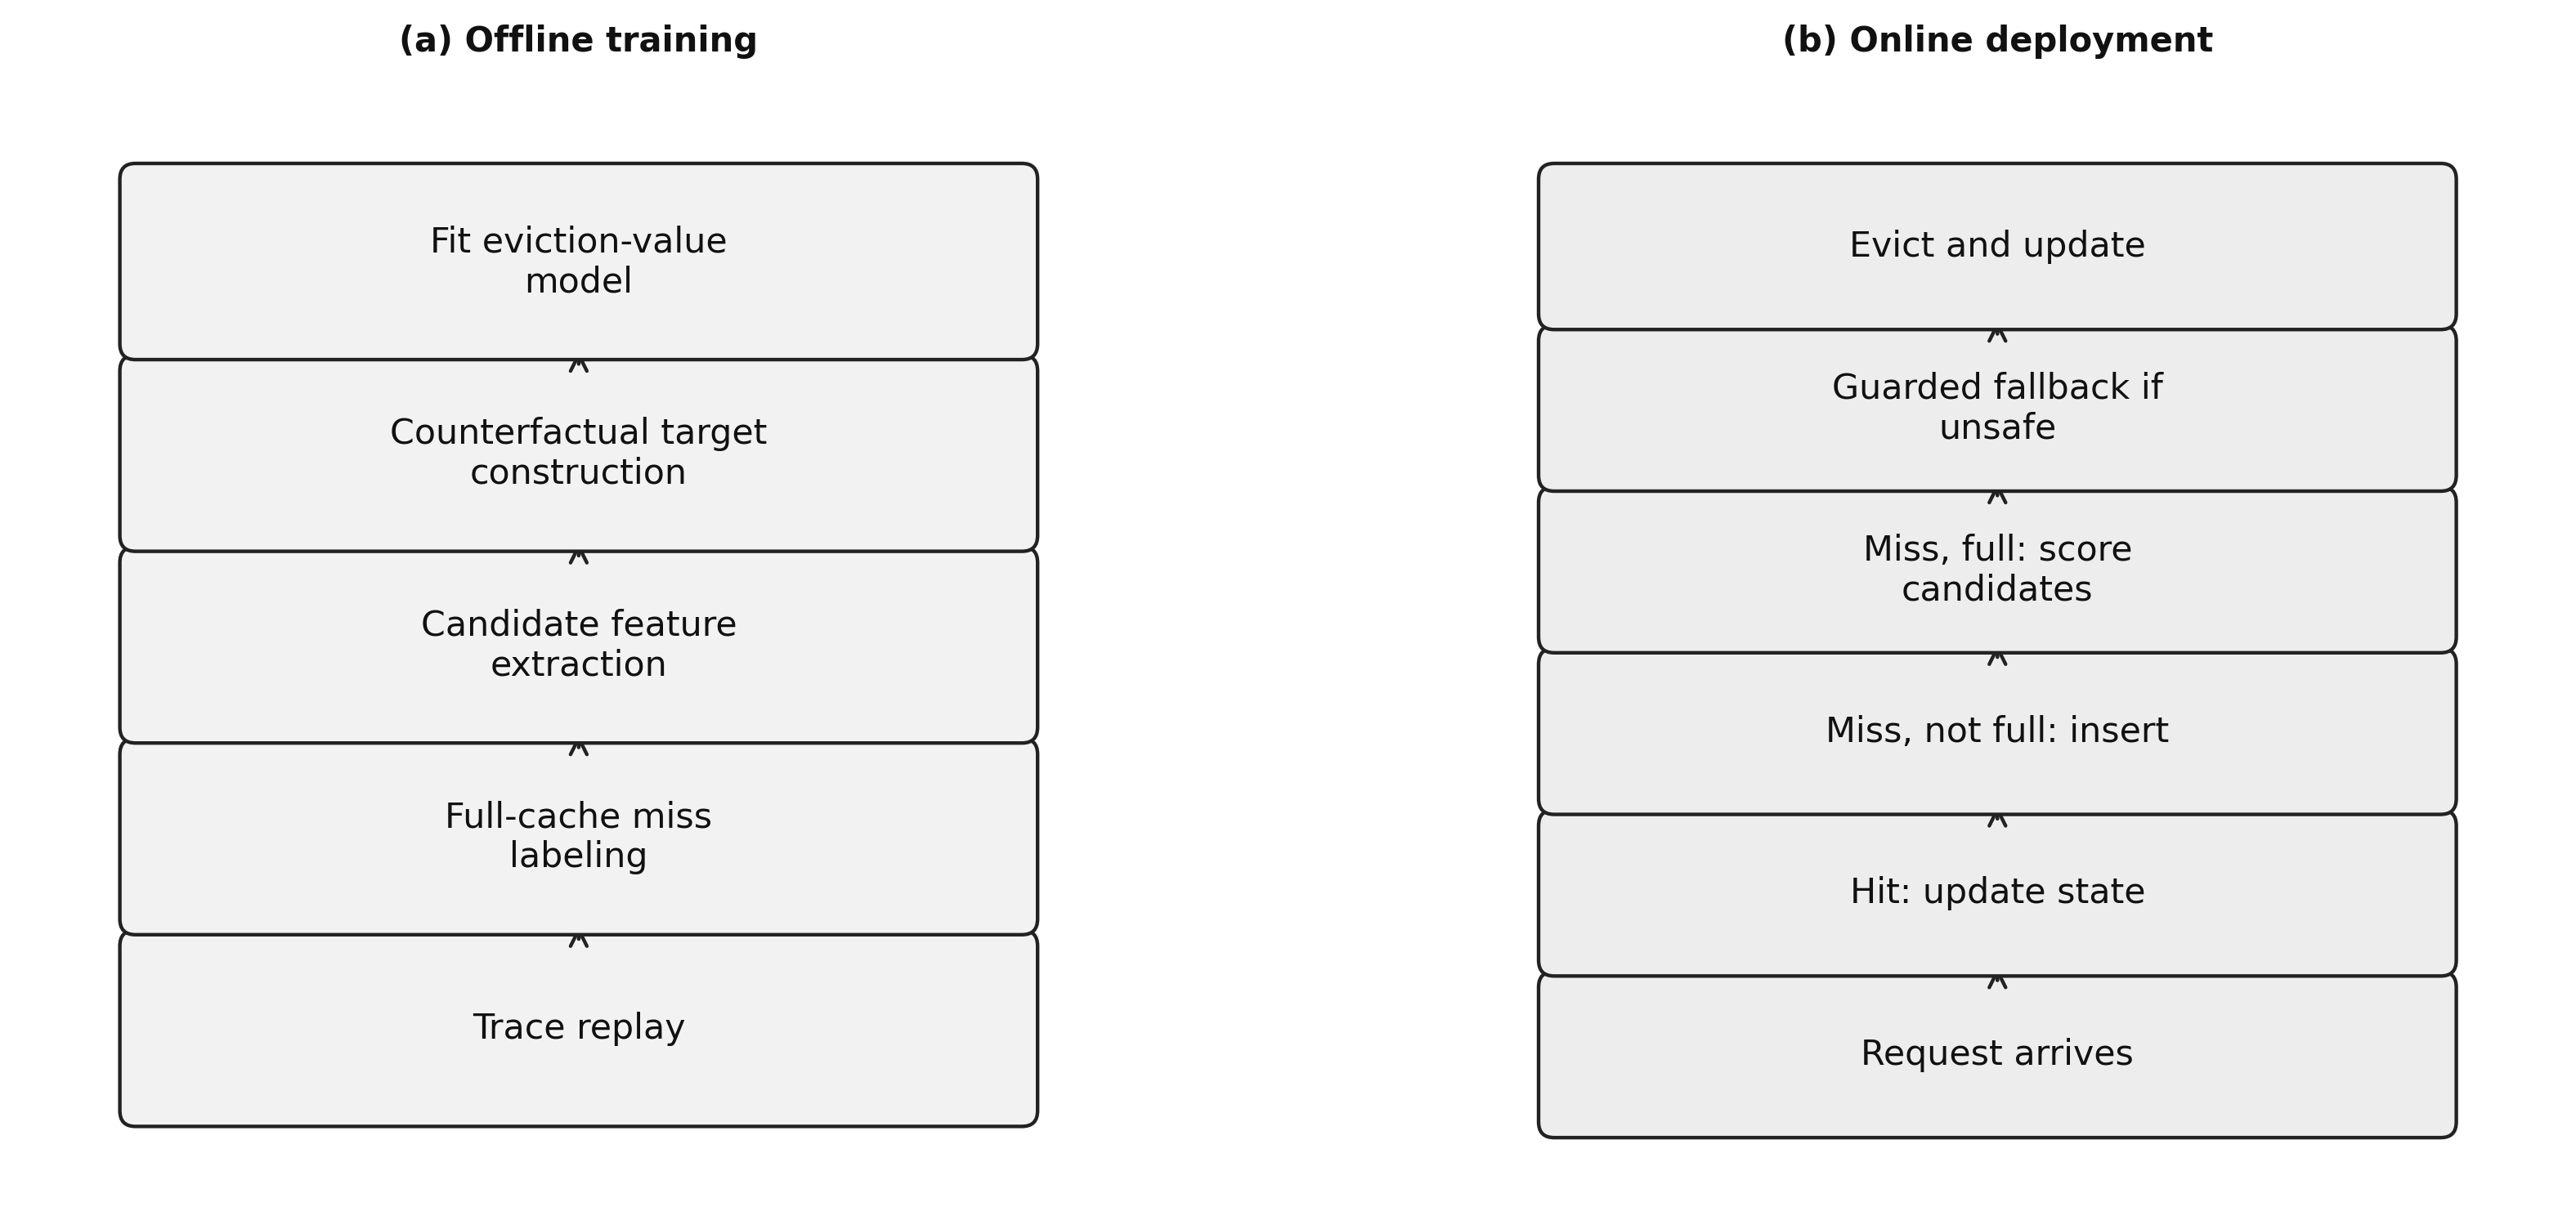
\includegraphics[width=0.96\textwidth]{figures/method_overview.png}
\caption{Conceptual overview of the eviction-value workflow. Offline replay is used to construct candidate-level training examples and finite-horizon loss targets, a supervised scorer is fitted to estimate decision-time eviction loss, and the online policy evicts the candidate with minimum predicted loss. An optional lightweight fallback layer can temporarily delegate control to a conservative baseline when repeated local signals indicate unsafe learned decisions.}
\label{fig:method_overview}
\end{figure*}

In the implementation studied here, candidate-level supervision is generated for the main eviction-value line, a scorer is trained for a chosen replay horizon, and the resulting policy is evaluated in the same simulator used for the reference baselines. The framework records aggregate metrics together with step-level logs so that downstream behavior can be analyzed jointly with fallback activity.

At decision time $t$, the method first builds the candidate feature matrix
\begin{equation}
X_t =
\begin{bmatrix}
x(q_1,t)^{\top}\\
x(q_2,t)^{\top}\\
\vdots\\
x(q_k,t)^{\top}
\end{bmatrix},
\label{eq:candidate_feature_matrix}
\end{equation}
where $\{q_1,\ldots,q_k\}=C_t$ is the current candidate set. The learned scorer then returns the vector of predicted losses
\begin{equation}
\widehat{\ell}_t =
\begin{bmatrix}
\widehat{L}_H(q_1,t)\\
\widehat{L}_H(q_2,t)\\
\vdots\\
\widehat{L}_H(q_k,t)
\end{bmatrix},
\label{eq:predicted_loss_vector}
\end{equation}
and the learned victim is selected by
\begin{equation}
q_t^{*} = \arg\min_{q_i \in C_t} \widehat{L}_H(q_i,t).
\label{eq:workflow_argmin}
\end{equation}
If the optional fallback controller is active, this proposal is passed through the mechanism described in the previous subsection before the final eviction is applied. Learned policies and baselines share the same simulator and trace-loading interface.

\section{Experiments and Discussion}
\label{sec:experiments}


\subsection{Experimental Setup}
\label{subsec:experimental_setup}

The experiments are designed to evaluate the proposed eviction-value framework under a controlled replay protocol. All policies are executed within a common simulator using the same processed traces, cache capacities, request ordering, and trace-loading interface. This unified execution setting is important because it reduces confounding from preprocessing differences, trace-format inconsistencies, and policy-specific replay semantics. Consequently, observed differences in performance can be attributed more directly to differences in eviction behavior.

The empirical focus is the main candidate-scoring policy, \texttt{evict\_value\_v1}, together with a selected set of classical, predictive, and robust reference policies from the learning-augmented caching literature \cite{lykouris2021competitive_caching,antoniadis2020online_metric_untrusted,wei2020better_simpler_lac,chledowski2021robust_lac_experimental}. These baselines are included because they represent the most relevant practical comparison points for online paging under imperfect predictive information. Other policy families implemented in the broader codebase are treated as exploratory or contextual comparisons and are not part of the main empirical claim unless their results are explicitly reported.

The evaluation has two complementary components. The first is \emph{offline scorer construction and selection}. In this component, candidate-level examples are generated from replayed eviction decisions, finite-horizon loss labels are constructed, and model families are compared using target-quality metrics that assess how well the learned scorer approximates the proposed supervision objective. The second is \emph{online replay evaluation}, in which the induced policy is executed in the same simulator as the reference baselines and compared through downstream replay performance. This separation is methodologically important because strong performance on an offline proxy does not necessarily translate into the best online replacement decisions once the scorer is embedded in the full decision loop.

To isolate the eviction-choice problem, the study is conducted in the standard unweighted paging setting with fixed cache capacity and unit miss cost. The principal downstream metric is therefore the total number of cache misses over the replayed request sequence. Claims are restricted to what is directly supported by the reported evaluation outputs below.

\subsection{Datasets, Baselines, and Evaluation Metrics}
\label{subsec:datasets-baselines-metrics}

The empirical study is organized around a common replay interface applied to heterogeneous request traces and a baseline pool chosen to reflect the most relevant practical comparison points for learning-augmented paging. Reported results are restricted to the artifact-backed trace, capacity, and policy subset instantiated by the designated evaluation pipeline.

The baseline pool is selected to cover five comparison roles: classical paging references, CLOCK-family structural references, predictive paging references, robust learning-augmented controllers, and directly comparable learned cache-replacement systems. Classical and CLOCK-family references include least-recently used eviction, SIEVE, and FIFO-Reinsertion, which remain essential lightweight anchors for unweighted online caching \cite{belady1966replacement_algorithms,fiat1991competitive_paging,zhang2024sieve}. Predictive and robust references include predictive marker, trust-and-doubt-style control, a regret-driven selective-trust gating controller (REST), and the blind-oracle/LRU combiner \cite{lykouris2021competitive_caching,antoniadis2020online_metric_untrusted,wei2020better_simpler_lac,chledowski2021robust_lac_experimental,im2022parsimonious_lac,rohatgi2020near_optimal_caching}. The learned cache-replacement role adds LRB, 3L-Cache, CACHEUS, and HALP \cite{song2020lrb,zhou2025threelcache,rodriguez2021cacheus,song2023halp}, providing the direct comparison against modern learned replacement systems reported in Section~\ref{subsec:major1_comparison}. These methods are used because they represent strong and practically relevant reference points when predictions are informative but imperfect.

Within the learned-policy family, the main method studied in this paper is \texttt{evict\_value\_v1}, which predicts a candidate-specific finite-horizon downstream eviction loss and evicts the candidate with minimum predicted loss. The framework also implements an optional guard that can temporarily defer to a conservative fallback policy when recent online behavior indicates locally unsafe learned decisions; this guard is an implementation safeguard evaluated only as an ablation in the present study, and we do not claim that it improves end-to-end miss ratio unless future experiments support it. Other policy families implemented in the repository, including a standalone marker-style policy, a robust follow-the-prediction combiner with marker fallback, pairwise-ranking variants, sentinel-style guards, and additional exploratory controllers, are retained for contextual analysis and ongoing research development, but they are not treated as central baselines for the present manuscript unless their results are explicitly reported in the canonical artifact bundle.

Table~\ref{tab:trace_families} summarizes the workload families relevant to the present study from a manuscript perspective. The table is intentionally phrased at the family level to separate source provenance from the narrower question of which canonical artifacts are currently reported. Table~\ref{tab:main_policy_families} summarizes the main policy families used in the empirical comparison.

\begin{table}[!htbp]
\centering
\caption{Trace families in the artifact-backed evaluation. The repository supports additional workloads; reported results are restricted to the canonical artifact subset.}
\label{tab:trace_families}
\small
\begin{tabular}{p{2.8cm} p{4.3cm} p{5.0cm}}
\hline
\textbf{Trace family} & \textbf{Representative source} & \textbf{Role in this work} \\
\hline
BrightKite & BrightKite mobility trace \cite{cho2011friendship_mobility} & Public request stream with heterogeneous locality structure for controlled replay evaluation. \\
Citi Bike & Citi Bike system data \cite{citibike_system_data} & Public event stream used to derive replayable request sequences under a common preprocessing interface. \\
SPEC CPU2006 & SPEC CPU2006 benchmark descriptions \cite{henning2006spec_cpu2006} & Classical systems-style trace family providing a contrasting locality regime. \\
Wikimedia pageviews & Wikimedia pageview dumps \cite{wikimedia_pageviews} & Large public page-access source for replay-based cache evaluation. \\
Production-style cache traces & Twitter cache clusters, SHARDS-related resources, and open cache-workload sources \cite{yang2020twitter_cache_clusters,waldspurger2015shards,cachemon_open_source_cache_dataset,cachelib_cachebench_fb_hw_eval} & Manifest-based or documented production-style workloads used to broaden workload diversity in the repository and, when artifact-backed, in the manuscript evaluation. \\
\hline
\end{tabular}
\end{table}

\begin{table}[!htbp]
\centering
\caption{Main policy families in the empirical comparison. A diagnostic-only blind-oracle variant used for internal sanity checks is excluded from the reported comparisons. LRB, 3L-Cache, CACHEUS, and HALP are evaluated only in the matched-protocol comparison of Section~\ref{subsec:major1_comparison}, not in the Section~\ref{subsec:end_to_end_capacities} eight-policy sweep, and are listed here for completeness of the full policy roster.}
\label{tab:main_policy_families}
\small
\begin{tabular}{p{2.2cm} p{2.3cm} p{6.6cm}}
\hline
\textbf{Label} & \textbf{Category} & \textbf{Role in evaluation} \\
\hline
LRU & Classical baseline & Standard recency-based eviction reference \cite{belady1966replacement_algorithms}. \\
SIEVE & Classical baseline & CLOCK-family turn-key eviction algorithm using a single FIFO queue and an advancing hand pointer over retained objects \cite{zhang2024sieve}. \\
FIFO-Reinsertion & Classical baseline & CLOCK / Second-Chance family baseline that reinserts a retained survivor at the head of the queue rather than advancing a hand \cite{zhang2024sieve}. \\
PredMk & Predictive baseline & Prediction-aware marker-style paging baseline \cite{lykouris2021competitive_caching}. \\
BO/LRU & Combiner baseline & Blind-oracle/LRU practical combiner baseline \cite{wei2020better_simpler_lac}. \\
T\&D & Robust baseline & Trust-and-doubt-style controller for untrusted predictions \cite{antoniadis2020online_metric_untrusted}. \\
REST & Heuristic baseline & Regret-driven selective-trust gating controller that switches between a predictor-driven eviction rule and an LRU fallback based on delayed online feedback. \\
LRB & Learned baseline & Belady-guided future-access learned eviction system for CDN caching; independent repository reimplementation \cite{song2020lrb}. \\
3L-Cache & Learned baseline & Low-overhead learned eviction policy using bidirectional candidate sampling; independent repository reimplementation \cite{zhou2025threelcache}. \\
CACHEUS & Learned baseline & Learned expert-mixture eviction controller; official-source-unmodified wrapper \cite{rodriguez2021cacheus}. \\
HALP & Learned baseline & Candidate-level preference learning from future re-access outcomes; independent reimplementation, no official public code exists \cite{song2023halp}. \\
EV & Proposed method & Candidate-level finite-horizon eviction-value predictor. \\
\hline
\end{tabular}
\end{table}

The primary evaluation metric is the total number of cache misses incurred during online replay. We also report hit rate and, where useful for interpretation, miss deltas relative to the LRU baseline. For offline scorer analysis, we additionally use target-quality diagnostics such as regret-style error summaries, Top-1 agreement, and disagreement-oriented statistics. These auxiliary quantities help interpret the learned scorer, but downstream replay performance remains the decisive criterion.

\subsection{Offline Ablation and Model Selection}
\label{subsec:main_results}

We begin with the offline ablation used to select the scorer configuration for \texttt{evict\_value\_v1}. Table~\ref{tab:evict-value-ablation} and Fig.~\ref{fig:evict-value-ablation} summarize validation and test regret across replay horizons and model families. These results are used to characterize the learnability of the candidate-level target and to motivate the scorer configuration carried into the main policy line.

Two patterns are clear. First, the nonlinear tree-based models are consistently stronger than the linear ridge baseline. Across all three replay horizons, ridge incurs substantially larger regret than either \texttt{hist\_gb} or \texttt{random\_forest}. This indicates that the eviction-value target is not well captured by a simple linear approximation and benefits from a more flexible scorer.

Second, shorter replay horizons are stronger in the current artifact set. Horizon $H=4$ gives the best validation regret for \texttt{hist\_gb} and the best test regret for \texttt{random\_forest}, while performance deteriorates as the horizon increases to $8$ and $16$. This trend is consistent with the intended role of the target: a shorter horizon appears to provide a cleaner and more learnable proxy for local eviction harm, whereas longer horizons introduce additional downstream interactions that are harder to model accurately.

The Top-1 results support the same interpretation. On both validation and test splits, the tree-based models achieve lower Top-1 error than ridge across the evaluated horizons, suggesting that nonlinear scorers preserve the candidate ordering needed for eviction decisions more effectively than a linear baseline. At the same time, the gap between \texttt{hist\_gb} and \texttt{random\_forest} is modest relative to their shared advantage over ridge. The main methodological conclusion is therefore about the value of nonlinear scoring and short-horizon supervision, not about one tree-based model being universally dominant.

Taken together, these ablation results support a conservative model-selection conclusion: within the current artifact-backed evidence, the candidate-level eviction-value framework is strongest with a short replay horizon and a nonlinear scorer. This evidence does not by itself establish superiority in end-to-end online replay, but it does show that the proposed target yields a meaningful and learnable signal for downstream eviction scoring.

\begin{table}[!htbp]
\centering
\caption{Offline ablation for \texttt{evict\_value\_v1} across replay horizons and model families. Lower regret is better, and lower Top-1 error is better.}
\label{tab:evict-value-ablation}
\small
\setlength{\tabcolsep}{5pt}
\begin{tabular}{r l r r r r}
\toprule
Horizon & Model & Val.\ regret & Test regret & Val.\ Top-1 & Test Top-1 \\
\midrule
4  & hist\_gb       & 0.0091 & 0.0055 & 0.0174 & 0.0316 \\
4  & random\_forest & 0.0134 & 0.0046 & 0.0154 & 0.0264 \\
4  & ridge          & 0.0649 & 0.0150 & 0.0503 & 0.0832 \\
8  & hist\_gb       & 0.0203 & 0.0104 & 0.0157 & 0.0362 \\
8  & random\_forest & 0.0240 & 0.0120 & 0.0177 & 0.0267 \\
8  & ridge          & 0.0880 & 0.0384 & 0.0377 & 0.0795 \\
16 & hist\_gb       & 0.0394 & 0.0196 & 0.0203 & 0.0365 \\
16 & random\_forest & 0.0431 & 0.0178 & 0.0157 & 0.0249 \\
16 & ridge          & 0.1166 & 0.0850 & 0.0277 & 0.0826 \\
\bottomrule
\end{tabular}
\end{table}

\begin{figure}[!htbp]
    \centering
    
\includegraphics[width=\columnwidth]{figures/figure4_ablation.png}
    \caption{Offline ablation for \texttt{evict\_value\_v1} across replay horizons and model families. The figure summarizes validation and test regret for the configurations shown in Table~\ref{tab:evict-value-ablation}. Lower is better.}
    \label{fig:evict-value-ablation}
\end{figure}

\subsection{End-to-End Online Replay Evaluation Across Available Capacities}
\label{subsec:end_to_end_capacities}

In addition to the offline ablation above, we report end-to-end online replay results for all eight policies in Table~\ref{tab:main_policy_families}, evaluated under the common simulator described in Section~\ref{subsec:experimental_setup} across the seven trace families in Table~\ref{tab:trace_families}, at 50{,}000 requests per trace. At the time of writing, this evaluation has been completed at cache capacities 32, 64, and 128 slots; capacity 256 has not yet been evaluated end-to-end and is not reported in this paper. We are explicit about this boundary because the capacity-128 result discussed below is itself non-monotonic relative to capacities 32 and 64, and we judged it more important to report and analyze the existing three-point trend honestly than to extend further computation into a larger capacity sweep before doing so.

Table~\ref{tab:available-capacities-trend} reports mean replay misses, averaged across the seven trace families, for each policy at each evaluated capacity, and Fig.~\ref{fig:available-capacities-trend} visualizes the same data together with \texttt{evict\_value\_v1}'s relative gap against the three strongest lightweight baselines (LRU, SIEVE, and FIFO-Reinsertion).

We disclose an important protocol limitation of this specific evaluation directly here rather than only in the Limitations section: the \texttt{evict\_value\_v1} model underlying Table~\ref{tab:available-capacities-trend} was fit with a chunk-level train/validation/test split applied within each trace's own full \texttt{[0, 50{,}000)} request range, rather than on a held-out trace family with zero overlap with the evaluated stream. This means the reported numbers for \texttt{evict\_value\_v1} in this specific table do not rule out train/test overlap and should not be read as a clean estimate of its generalization performance; the seven non-learned or fixed reference policies in this table (LRU, SIEVE, FIFO-Reinsertion, PredMk, T\&D, BO/LRU, REST) are unaffected, since they are either parameter-free or do not fit trace-specific models on this data. Section~\ref{subsec:major1_comparison} reports a corrected, leakage-free evaluation of \texttt{evict\_value\_v1} using leave-one-family-out training, together with the direct comparison against LRB, 3L-Cache, CACHEUS, and HALP requested for this revision; that corrected evaluation is the primary evidence for \texttt{evict\_value\_v1}'s comparative performance in this paper. We retain Table~\ref{tab:available-capacities-trend} because it is the only evaluation in this paper covering PredMk, T\&D, BO/LRU, and REST, and because, notably, the potential overlap did not produce a favorable bias here: \texttt{evict\_value\_v1} still underperforms every other policy in this table despite it.

\begin{table}[!htbp]
\centering
\caption{End-to-end online replay evaluation: mean misses across the seven trace families in Table~\ref{tab:trace_families} (50{,}000 requests/trace), at each evaluated cache capacity. Capacity 256 has not yet been evaluated end-to-end.}
\label{tab:available-capacities-trend}
\small
\begin{tabular}{l r r r}
\toprule
Policy & Cap.\ 32 & Cap.\ 64 & Cap.\ 128 \\
\midrule
LRU              & 34667.1 & 33650.1 & 32495.6 \\
SIEVE             & 35313.6 & 34362.7 & 33279.3 \\
FIFO-Reinsertion  & 34688.0 & 33672.1 & 32530.6 \\
PredMk            & 34843.9 & 33773.1 & 32664.6 \\
T\&D              & 35087.0 & 33998.7 & 32928.9 \\
BO/LRU            & 34668.6 & 33651.3 & 32496.9 \\
REST              & 34667.1 & 33650.1 & 32495.6 \\
EV (proposed)     & 36344.1 & 34409.0 & 36316.6 \\
\bottomrule
\end{tabular}
\end{table}

\begin{figure}[!htbp]
\centering
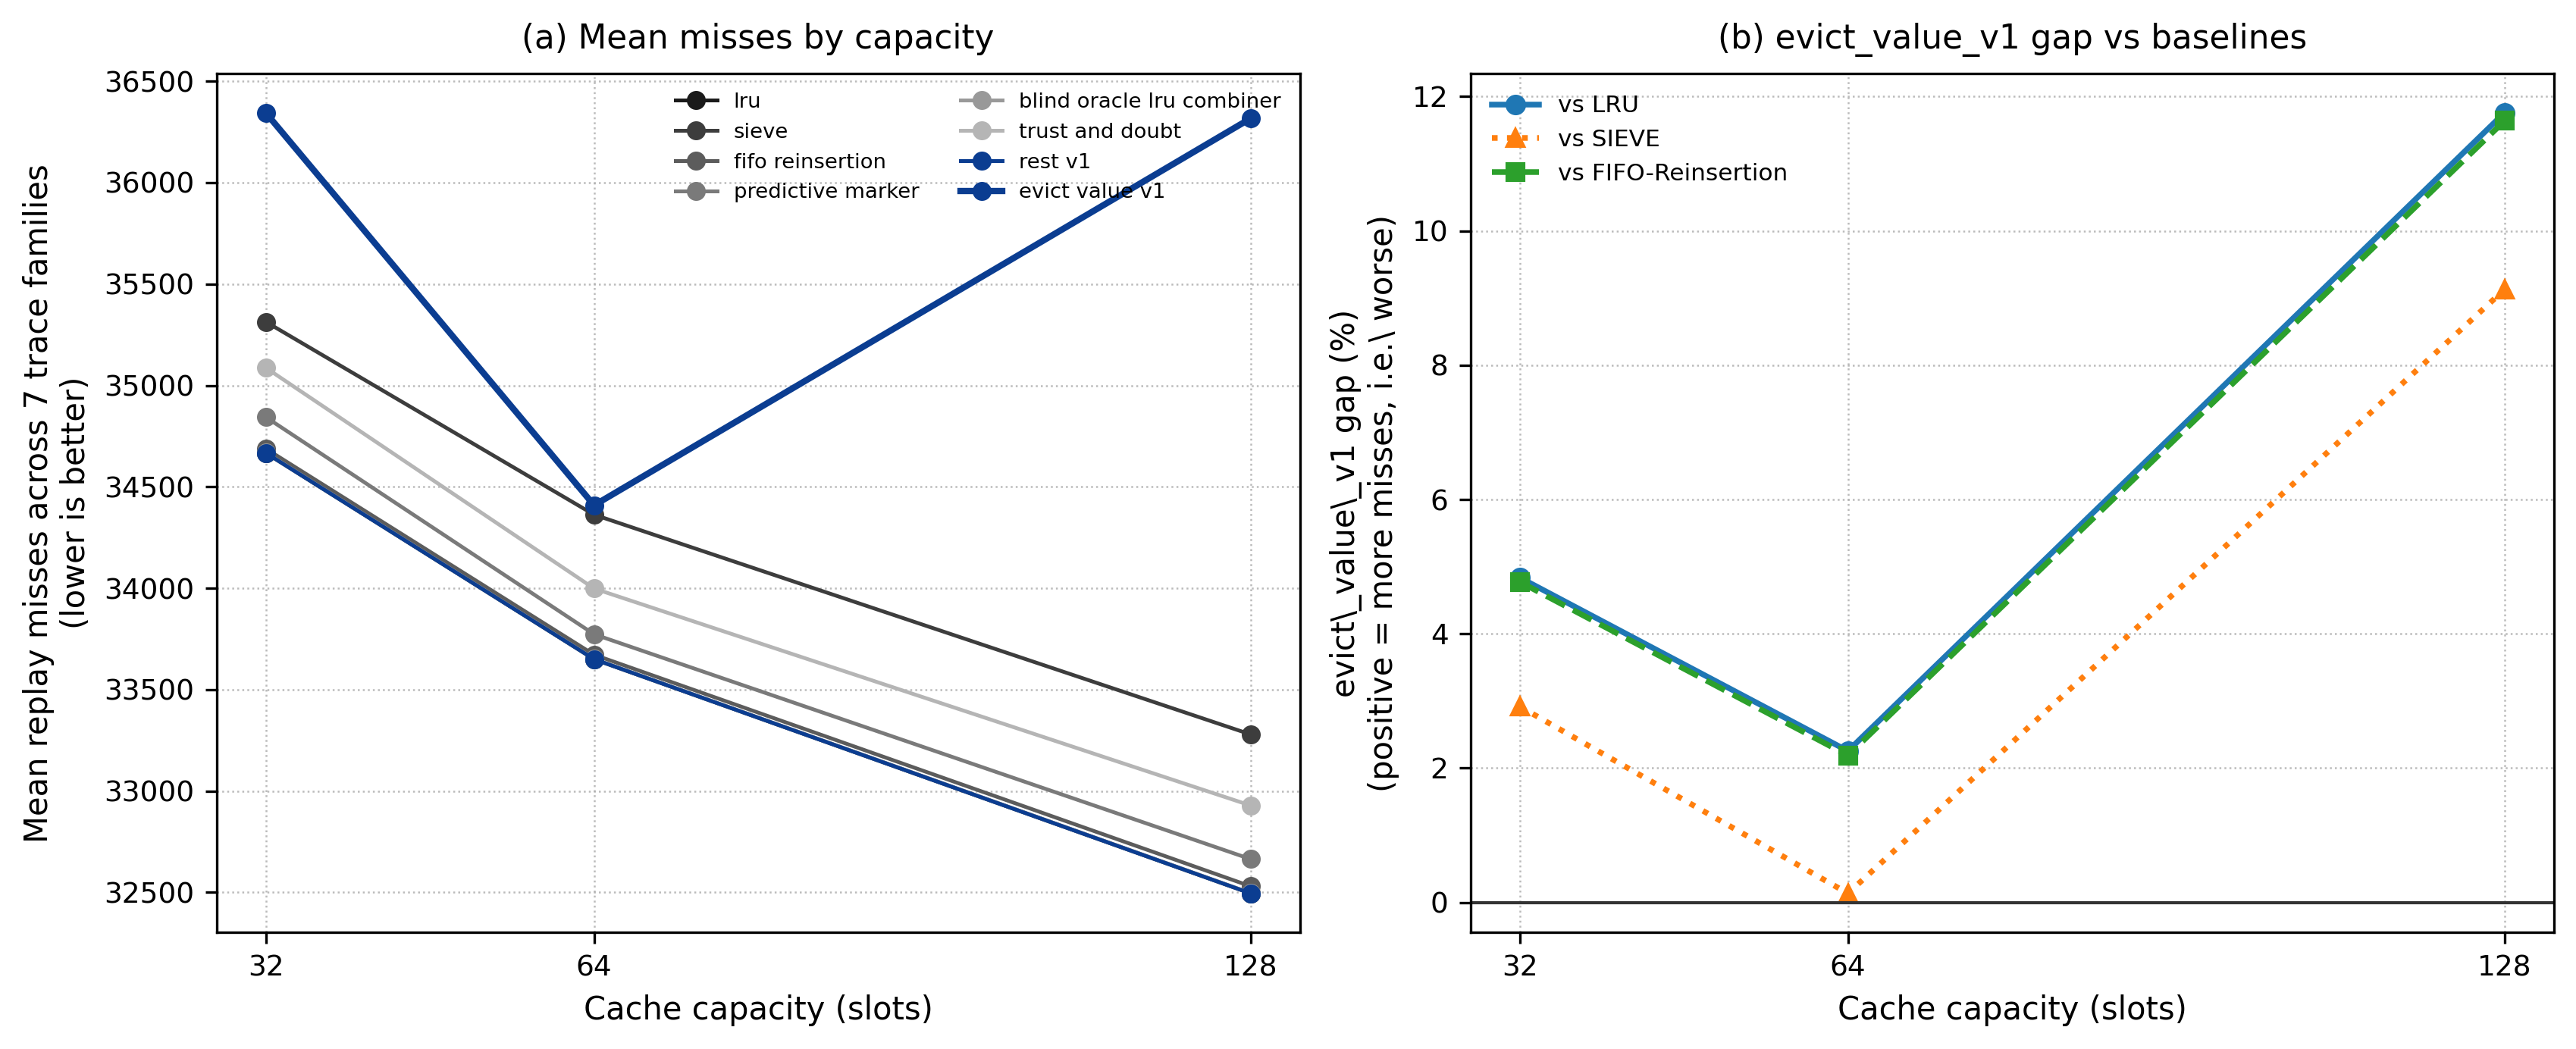
\includegraphics[width=\linewidth]{figures/figure_available_capacities_trend.png}
\caption{Capacity-trend comparison across the available evaluated capacities (32, 64, 128; capacity 256 not evaluated in this revision). (a) Mean replay misses per policy at each capacity, averaged across the seven trace families. (b) \texttt{evict\_value\_v1}'s relative miss gap against LRU, SIEVE, and FIFO-Reinsertion at each capacity; positive values indicate more misses than the baseline. The LRU and FIFO-Reinsertion gap curves nearly coincide because the two baselines have nearly identical miss counts in the averaged replay; distinct line styles and markers are used to keep them visually separable. The non-monotonic widening at capacity 128 is discussed in Section~\ref{subsec:discussion_analysis} and Section~\ref{subsec:limitations}.}
\label{fig:available-capacities-trend}
\end{figure}

Three observations follow directly from this available-capacity replay. First, \texttt{evict\_value\_v1} does not improve on LRU, SIEVE, FIFO-Reinsertion, or REST on average at any of the three evaluated capacities: its mean-miss gap relative to LRU is $+4.84\%$ at capacity 32, $+2.26\%$ at capacity 64, and $+11.76\%$ at capacity 128 (equivalently $+2.92\%$, $+0.13\%$, and $+9.13\%$ against SIEVE, and $+4.77\%$, $+2.19\%$, and $+11.64\%$ against FIFO-Reinsertion). REST is numerically tied with LRU at all three evaluated capacities, so the same average gap applies there as well. This is a negative end-to-end result for the proposed policy relative to the strongest baselines in our pool, and we report it directly rather than restricting the paper's empirical claims to the offline ablation evidence above.

Second, the other reference policies cluster tightly around LRU at every evaluated capacity. \texttt{blind\_oracle\_lru\_combiner} (BO/LRU) and \texttt{rest\_v1} (REST) are numerically indistinguishable from LRU ($0.00\%$ gap) at all three capacities, FIFO-Reinsertion stays within $0.11\%$ of LRU throughout, and SIEVE, T\&D, and PredMk remain within roughly $0.4$--$2.4\%$ of LRU at every capacity. \texttt{evict\_value\_v1} is the only policy in the comparison whose gap exceeds $5\%$ at any evaluated capacity, and the only one whose relative position worsens between capacity 64 and capacity 128 rather than tracking the otherwise stable ordering of the other seven policies.

Third, the capacity trend for \texttt{evict\_value\_v1} is non-monotonic: the gap narrows from capacity 32 to capacity 64 and then widens sharply at capacity 128, rather than improving or degrading smoothly with capacity. We examine this pattern at the workload level next, and return to its likely cause in the Discussion and Limitations.

\subsection{Workload-Specific Breakdown}
\label{subsec:workload_breakdown}

Table~\ref{tab:family-capacity-gap} reports \texttt{evict\_value\_v1}'s relative miss gap against LRU separately for each of the seven trace families at each evaluated capacity, rather than only as the family-averaged numbers in Table~\ref{tab:available-capacities-trend}.

\begin{table}[!htbp]
\centering
\caption{\texttt{evict\_value\_v1} relative miss gap against LRU, by trace family and evaluated capacity. Positive values indicate more misses than LRU (worse).}
\label{tab:family-capacity-gap}
\small
\begin{tabular}{l r r r}
\toprule
Trace family & Cap.\ 32 & Cap.\ 64 & Cap.\ 128 \\
\midrule
BrightKite    & $+10.47\%$ & $+10.72\%$ & $+50.91\%$ \\
Citi Bike     & $+7.90\%$  & $+4.70\%$  & $+45.49\%$ \\
CloudPhysics  & $+0.72\%$  & $+1.57\%$  & $+3.10\%$ \\
MetaCDN       & $+22.37\%$ & $+2.73\%$  & $+17.62\%$ \\
MetaKV        & $+1.70\%$  & $+0.01\%$  & $+0.76\%$ \\
Twemcache     & $+1.84\%$  & $+3.16\%$  & $+14.06\%$ \\
Wikimedia$^\dagger$ & $+0.00\%$  & $+0.00\%$  & $+0.00\%$ \\
\bottomrule
\end{tabular}
\\[3pt]
\footnotesize $^\dagger$Degenerate at every evaluated capacity: all eight policies reach 50{,}000/50{,}000 misses (0\% hit rate), because the working set exceeds even the largest evaluated capacity. Not informative for cross-policy comparison.
\end{table}

Two patterns stand out. First, Wikimedia pageviews is degenerate at every evaluated capacity, as noted in the table, and we exclude it from substantive interpretation. CloudPhysics and MetaKV remain close to LRU at every capacity (at most $+3.10\%$ and $+1.70\%$, respectively), consistent with the family-averaged picture in Table~\ref{tab:available-capacities-trend}.

Second, the capacity-128 widening is concentrated in, but not limited to, two families. BrightKite and Citi Bike show the largest gaps at capacity 128 ($+50.91\%$ and $+45.49\%$, respectively), up sharply from roughly $+10\%$ or less at capacities 32 and 64. MetaCDN and Twemcache also show double-digit gaps at capacity 128 ($+17.62\%$ and $+14.06\%$), though their capacity-32/64 trajectories differ from BrightKite's and Citi Bike's: MetaCDN's gap is actually largest at capacity 32 ($+22.37\%$), drops to $+2.73\%$ at capacity 64, and rises again at capacity 128, a U-shaped pattern rather than a monotonic one, while Twemcache's gap increases steadily across all three capacities ($+1.84\%$, $+3.16\%$, $+14.06\%$). In total, four of the six non-degenerate families show a capacity-128 gap above $10\%$, while the remaining two (CloudPhysics, MetaKV) stay below $3.1\%$ throughout. We therefore describe the capacity-128 degradation as broad-based rather than as an artifact specific to two outlier traces, while still noting that BrightKite and Citi Bike are the most extreme cases.

Taken together with the offline ablation in Section~\ref{subsec:main_results}, the capacity-128 degradation documented above is broad-based across workload families rather than an artifact of a single outlier trace, reinforcing rather than qualifying away the negative end-to-end result already reported in Section~\ref{subsec:end_to_end_capacities}. We discuss its likely cause in Section~\ref{subsec:discussion_analysis} and revisit it in Section~\ref{subsec:limitations}.

\subsection{Matched Comparison Against Learned Cache-Replacement Baselines}
\label{subsec:major1_comparison}

This section reports a corrected, leakage-free evaluation of \texttt{evict\_value\_v1} and directly compares it against four learned cache-replacement systems -- LRB, 3L-Cache, CACHEUS, and HALP -- alongside LRU, SIEVE, and FIFO-Reinsertion, addressing both the train/test-overlap limitation disclosed in Section~\ref{subsec:end_to_end_capacities} and the request for a direct comparison with existing learned methods, particularly LRB and 3L-Cache.

\subsubsection{Corrected training protocol}

\texttt{evict\_value\_v1} is retrained under a leave-one-family-out protocol: for each of the seven trace families in turn, the model is trained only on the other six (five for training, one for validation-only hyperparameter selection), and the held-out family contributes zero rows to training, validation, hyperparameter selection, feature selection, horizon selection, seed selection, or early stopping at any point before the model is frozen and evaluated. This removes the train/test overlap present in the model underlying Table~\ref{tab:available-capacities-trend} by construction, since a held-out family's own requests never appear anywhere in its own model's training pipeline.

\subsubsection{Matched evaluation protocol}

All eight policies compared in this section -- \texttt{evict\_value\_v1} and the seven baselines -- are evaluated on identical inputs: the same seven request traces (verified by SHA-256 hash, not filename), cache capacities 32, 64, and 128 under identical object-slot capacity and unit-object-size semantics, an identical history prefix \texttt{[0, 10{,}000)}, an identical scored suffix \texttt{[10{,}000, 50{,}000)} (40,000 scored requests), and identical hit/miss accounting. We emphasize that \emph{matched evaluation protocol} refers only to these evaluation-side inputs and does not imply identical training or adaptation procedures: LRB, 3L-Cache, and CACHEUS are online/adaptive baselines that learn continuously from their own in-trace stream with no cross-family training corpus at all; HALP is trained offline but only on each trace's own history prefix; LRU, SIEVE, and FIFO-Reinsertion are parameter-free; and \texttt{evict\_value\_v1} is trained offline with the leave-one-family-out procedure above. No baseline in this comparison, including \texttt{evict\_value\_v1}, has access to future request information or to another family's data at any point.

\subsubsection{Results}

Table~\ref{tab:major1-comparison} reports, for each baseline, the mean miss ratio over the 21 matched (family, capacity) cells, the number of cells \texttt{evict\_value\_v1} wins, loses, and ties against that baseline, and the relative mean difference in miss ratio. \texttt{evict\_value\_v1}'s own mean primary miss ratio across all 21 cells is $0.700463$.

\begin{table}[!htbp]
\centering
\caption{Matched-protocol comparison of \texttt{evict\_value\_v1} against learned and classical cache-replacement baselines, 21 (family, capacity) cells per baseline. Positive relative difference indicates \texttt{evict\_value\_v1} has a higher (worse) mean miss ratio than the baseline. LRB, 3L-Cache, CACHEUS, and HALP are learned baselines; LRU, SIEVE, and FIFO-Reinsertion are classical.}
\label{tab:major1-comparison}
\small
\begin{tabular}{l r r r r r}
\toprule
Baseline & Baseline mean & EV wins & Baseline wins & Ties & Rel.\ diff.\ \\
\midrule
LRB              & 0.6877 & 5 & 13 & 3 & $+1.85\%$ \\
3L-Cache          & 0.6926 & 5 & 13 & 3 & $+1.13\%$ \\
CACHEUS           & 0.6756 & 3 & 15 & 3 & $+3.68\%$ \\
HALP              & 0.6762 & 1 & 17 & 3 & $+3.59\%$ \\
LRU               & 0.6728 & 1 & 16 & 4 & $+4.12\%$ \\
SIEVE             & 0.6875 & 4 & 14 & 3 & $+1.89\%$ \\
FIFO-Reinsertion  & 0.6733 & 2 & 16 & 3 & $+4.04\%$ \\
\bottomrule
\end{tabular}
\end{table}

Under this matched comparison, \texttt{evict\_value\_v1} does not outperform any of the seven baselines: it loses on a clear majority of the 21 matched cells against every one (13--17 losses, 1--5 wins, 3--4 ties), with a positive (worse) mean relative miss-ratio difference ranging from $+1.13\%$ (3L-Cache) to $+4.12\%$ (LRU). This directly answers the request for a fair comparison against LRB and 3L-Cache: the comparison shows that \texttt{evict\_value\_v1} does not offer an empirical advantage over either under matched evaluation.

\subsubsection{Implementation-fidelity caveats}

LRB and 3L-Cache are independent repository reimplementations of their respective published algorithms, evaluated under the exact matched protocol above; 3L-Cache uses a fixed default batch size not re-tuned for this study, which we record as a material implementation caveat on its comparison. CACHEUS is executed via an official-source-unmodified wrapper around the authors' own released decision engine, with a provenance caveat that the external upstream clone is not currently live-verifiable in the present verification environment; this is a source-authenticity caveat, not an evaluation-input caveat. HALP is an independent reimplementation of the published method, since no official public HALP implementation exists; we treat it as a lower-fidelity supporting comparison rather than a primary result, consistent with Reviewer \#3's specific request for differentiation from HALP rather than an official empirical baseline. None of these caveats affect the matched-evaluation-protocol dimensions in Table~\ref{tab:major1-comparison}; they affect only how faithfully each reimplementation reproduces its source algorithm's exact behavior.

\subsection{Direct Comparison Against Alternative Supervision Objectives}
\label{subsec:objective_comparison}

Section~\ref{subsec:eviction_value_framework} motivates the finite-horizon eviction-loss target on the grounds that it is defined directly at the eviction decision, in contrast to indirect proxies such as reuse distance, next-arrival time, or pairwise candidate preference. This premise is testable, and we test it directly rather than argue for it only conceptually.

Using the same leave-one-family-out training and matched evaluation protocol as Section~\ref{subsec:major1_comparison}, we train and evaluate three alternative candidate-level supervision objectives in place of eviction-loss, holding the horizon, model family, feature set, and every other pipeline component fixed: a reuse-distance target (candidate-specific time to next reuse), a next-arrival target (candidate-specific time to the next request for that item), and a pairwise-preference target (candidate-specific relative ranking rather than an absolute value). Table~\ref{tab:objective-comparison} reports total misses over the 21 matched primary cells for each of the four objectives, including the proposed eviction-loss target.

\begin{table}[!htbp]
\centering
\caption{Supervision-objective comparison under the matched leave-one-family-out protocol, 21 primary cells, total misses (lower is better).}
\label{tab:objective-comparison}
\small
\begin{tabular}{l r r}
\toprule
Objective & Total misses & Mean miss ratio \\
\midrule
Eviction loss (proposed)  & 601{,}569 & 0.7162 \\
Next arrival              & 573{,}059 & 0.6822 \\
Reuse distance             & 571{,}456 & 0.6803 \\
Pairwise preference        & 565{,}127 & 0.6728 \\
\bottomrule
\end{tabular}
\end{table}

The proposed eviction-loss objective is the worst of the four alternatives, and it is the single worst objective within every one of the seven trace families individually (in the degenerate Wikimedia family, all four objectives tie at full misses), not merely on average. This directly contradicts the premise, stated in Section~\ref{subsec:eviction_value_framework} and implicit in the paper's original framing, that decision-aligned finite-horizon eviction-loss supervision is inherently better matched to the eviction decision than these indirect alternatives. We report this negative result plainly: within the tested horizon and model family, eviction-loss is not the strongest available finite-horizon candidate-level target, and pairwise preference -- despite not directly modeling downstream miss count -- performs best among the four. Section~\ref{subsec:mechanistic_diagnosis} investigates why the eviction-loss target underperforms, rather than simply reporting that it does.

\subsection{Mechanistic Diagnosis of the Eviction-Loss Target}
\label{subsec:mechanistic_diagnosis}

Sections~\ref{subsec:major1_comparison} and~\ref{subsec:objective_comparison} establish that \texttt{evict\_value\_v1} underperforms both external baselines and alternative supervision objectives. This section asks \emph{why}, using three targeted diagnostics run under the same matched protocol and the same 21 (family, capacity) cells. We organize the diagnosis as a sequence of questions, each answered by a specific measurement rather than by argument.

\textbf{Is inaccurate prediction the cause?} If the learned scorer poorly approximated the eviction-loss target, that alone would explain poor downstream performance. We test this by comparing the learned policy's decisions against an \emph{exact} solver for the same target (a per-decision oracle that computes the true horizon-4 eviction loss for every candidate directly, rather than a learned approximation). Across the 21 cells, the learned scorer's decisions agree with the exact target's optimal candidate set in $97.53\%$ of decisions (macro mean set-aware agreement across cells), with a mean target regret of $0.0247$ and a positive-regret fraction of $0.0247$; total learned misses ($601{,}569$) are within $6.4\%$ of the LRU reference ($565{,}126$) despite this near-perfect target agreement. This disfavors gross model-fitting failure as the primary explanation: the learned scorer is doing what it is asked to do.

\textbf{Is the target itself useful, even if perfectly optimized?} We answer this directly by replaying the exact horizon-4 oracle itself online, rather than a learned approximation of it. Across the same 21 cells, the exact oracle has a mean miss ratio of $0.770090$, compared to $0.672769$ for LRU -- the oracle loses to LRU on 18 of 21 cells, ties on 3, and never wins, with a mean cell-level disadvantage of $+0.0973$. This is the central diagnostic finding of this section: even \emph{perfect} optimization of the proposed horizon-4 eviction-loss target performs worse than LRU online. The problem is therefore not primarily one of approximation quality; it is that the target itself, at this horizon, does not correspond to a good online eviction policy.

\textbf{Why does the target fail even when optimized exactly?} We audit the target's decision-level structure directly. Across the same 21 cells, no decision ever has a unique optimal eviction candidate (unique-winner fraction $0.0$); every decision has multiple tied-optimal candidates (multiple-optimum fraction $1.0$); in $76.4\%$ of decisions every resident candidate is exactly tied for optimal (all-candidates-tied fraction); and on average $99.5\%$ of resident candidates fall within the optimal set (mean optimal-set fraction $0.9949$). The horizon-4 target is therefore severely degenerate: it almost never provides a strict, informative preference among the cached candidates, so the specific eviction choice a learned or exact policy makes among the many tied-optimal candidates is effectively unconstrained by the target, yet still determines downstream performance. A companion diagnostic quantifies the underlying cause: across $41{,}615{,}776$ candidate-residency observations at $565{,}126$ decision points, the probability that an item's true reuse time exceeds the 4-step horizon is $0.9939$ overall and $0.9793$ even conditioned on the item eventually being reused. The horizon-4 window observes only a small fraction of the reuse behavior that determines whether an eviction was actually costly, which is consistent with -- and offers a mechanistic explanation for -- the observed target degeneracy: most candidates' true consequences fall outside the window the target can see, so the target frequently cannot distinguish them.

\textbf{Summary.} A separate learning-curve check across five training-set fractions from 1\% to 50\% of the available candidate-level examples shows no material improvement in target-quality metrics with additional data, disfavoring insufficient training data (Section~\ref{subsec:main_results}'s offline ablation already selects the best-performing configuration within this data regime). Taken together with the agreement, oracle, and degeneracy diagnostics above, these results disfavor both insufficient training data and gross model-fitting failure, and instead identify severe target degeneracy, driven by horizon truncation relative to typical reuse timescales, as the dominant explanation for why the eviction-loss target underperforms both external baselines (Section~\ref{subsec:major1_comparison}) and alternative objectives (Section~\ref{subsec:objective_comparison}). Section~\ref{subsec:discussion_analysis} next examines a secondary, partial contributor: the mismatch between the label-construction continuation rule and the policy's own deployed trajectory.

\subsection{Discussion and Analysis}
\label{subsec:discussion_analysis}

The present results are most informative when interpreted through the central modeling choice of the paper: the proposed method is organized around a decision-aligned supervision target for candidate-level eviction scoring rather than around a global trust-calibration rule. This distinction is important because cache replacement is inherently a local comparative decision. At a full-cache miss, the policy must decide which currently cached item is least harmful to remove, not merely whether predictive information should be trusted in the abstract. From this perspective, the most direct question is not whether the advice appears accurate in isolation, but whether the learned target helps rank the available eviction candidates in a way that improves the actual online choice.

Viewed in this way, the main contribution of the current results is methodological. The offline ablation indicates that replay-based candidate supervision provides a meaningful route for translating predictive context into eviction decisions; tree-based scorers consistently outperform the linear ridge baseline across replay horizons, supporting candidate-level downstream supervision as a viable learning target.

The replay-horizon analysis provides a second useful insight. Within the current artifact set, shorter replay horizons yield the strongest regret values, with $H=4$ performing best among the evaluated settings, consistent with the intended interpretation that longer horizons incorporate harder-to-model downstream interactions.

More broadly, these findings suggest that supervision-target design deserves attention comparable to that given to the predictive signal itself. A candidate-level downstream-loss target remains a proxy, but it is defined directly at the decision point, which gives it a clearer operational interpretation than a trust score or an indirect action surrogate.

At the same time, the interpretation of these results should remain cautious, and the end-to-end evaluation in Section~\ref{subsec:end_to_end_capacities} sharpens rather than removes that caution. The replay-based loss studied here is finite-horizon and local rather than globally optimal, and the offline scorer-selection ablation does not by itself establish superiority in full end-to-end online replay. The explicit end-to-end evidence we now report directly answers that question, and the answer is negative: across all three evaluated capacities, \texttt{evict\_value\_v1} incurs more replay misses than LRU, SIEVE, and FIFO-Reinsertion, with the gap widening sharply and non-monotonically at capacity 128. Likewise, the broader framework includes guarded variants whose end-to-end effect remains unmeasured in the present study (see Limitations). The current results therefore support the proposed supervision target and scoring formulation as a learnable and well-motivated way to pose the eviction-decision problem, but they do not support a claim of downstream competitiveness, robustness across workload regimes, or effective fallback control in deployment; on the contrary, the end-to-end evidence weighs against competitiveness at every capacity evaluated so far.

A natural question is why a learnable, decision-aligned offline target would translate into a policy that underperforms strong baselines online, and whether the specific continuation-rule assumption used to build the supervision target contributes to this gap. Section~\ref{subsec:mechanistic_diagnosis} already establishes target degeneracy and horizon truncation as the dominant explanation; here we report a controlled causal test of a second, previously speculative hypothesis raised in an earlier version of this study: that the eviction-loss label's fixed LRU-style continuation assumption diverges from the policy's own recursive, non-LRU deployment trajectory, and that this divergence contributes to the observed gap.

We test this directly with a three-arm causal ablation under the leave-one-family-out protocol, isolating exactly one change between arms. \emph{C0} replays LRU end-to-end (the reference). \emph{C1} trains a policy $\pi_1$ on labels built under LRU continuation (matching Eq.~\eqref{eq:eviction_loss} as originally specified) and deploys $\pi_1$ recursively. \emph{C2} trains a second policy $\pi_2$ on labels built under a corrected continuation rule -- the frozen $\pi_1$'s own decisions, rather than LRU -- and deploys $\pi_2$ recursively; this is the only change between C1 and C2. Across the 21 (family, capacity) cells, C2 improves over C1 in 13 cells, ties in 3 (the degenerate Wikimedia cells), and worsens in 5, with a macro mean miss-ratio improvement of $-0.0102$; aggregate misses move from $601{,}569$ (C1) to $592{,}970$ (C2), against a $565{,}126$-miss LRU reference (C0). The improvement is not uniform: one cell, BrightKite at capacity 32, regresses sharply ($+0.2433$), which by itself prevents a claim of uniform benefit. We therefore classify the continuation-mismatch hypothesis as \emph{partially supported and regime-dependent}: correcting the continuation-label mismatch helps in most but not all family/capacity combinations, and is a real but secondary and non-uniform contributor to the gap documented in Sections~\ref{subsec:major1_comparison}--\ref{subsec:mechanistic_diagnosis}, not a full explanation of it.

A related but distinct question is whether the broader training-state distribution -- not just the continuation label itself -- diverging from the deployment-time trajectory is the operative mechanism, and whether correcting it helps. We test this with a one-step DAgger-style intervention that retrains on a mixture of on-policy and off-policy states to reduce a generic measured state-visitation shift index, holding everything else fixed. Across the same 21 cells, this intervention reduces the measured shift index in 16 of 21 cells, yet online misses improve in only 2, tie in 3, and worsen in 16, with a macro mean miss-ratio degradation of $+0.0094$ (aggregate misses $591{,}604 \to 599{,}537$). In 13 of the 18 informative (non-degenerate) cells, the shift metric improves while misses simultaneously worsen. We report this as a clear negative result for this specific intervention: reducing this generic, DAgger-style measure of state-distribution shift does not, by itself, improve online performance, even though the shift-reduction mechanism functions as intended on its own metric. This does not mean distribution shift does not exist as a phenomenon; it means that this particular corrective intervention, targeting a generic shift measure rather than the decision-relevant continuation label specifically, is not an effective remedy in the tested setting.

Taken together, the artifact-backed evidence supports a clear but negative conclusion about the present instantiation of the eviction-loss target, together with a well-supported mechanistic account of why. Finite-horizon candidate-level scoring, as a general framework for translating predictive context into eviction decisions, remains methodologically motivated, and short-horizon nonlinear scorers are the strongest configuration within the offline ablation for the eviction-loss target specifically (Section~\ref{subsec:main_results}). However, the eviction-loss target itself is not the strongest available choice within this framework: it loses to reuse-distance, next-arrival, and pairwise-preference alternatives under matched evaluation (Section~\ref{subsec:objective_comparison}), it does not outperform any of seven classical or learned baselines under a leakage-free matched comparison (Section~\ref{subsec:major1_comparison}), and even an exact oracle for the target performs worse than LRU online (Section~\ref{subsec:mechanistic_diagnosis}). We no longer treat the underlying cause as unconfirmed: severe target degeneracy at the tested horizon, driven by horizon truncation relative to typical reuse timescales, is the best-supported explanation, with continuation-label mismatch contributing a real but partial, regime-dependent secondary effect, and generic distribution-shift correction offering no remedy on its own. We therefore characterize \texttt{evict\_value\_v1}, in its present form, as a decision-aligned supervision study whose central target has been directly tested and found wanting, rather than as a practically superior online policy or even as the strongest available instantiation of its own framework. LRU, SIEVE, FIFO-Reinsertion, LRB, 3L-Cache, CACHEUS, and HALP all remain baselines the proposed method does not currently outperform under matched evaluation. Future work on this framework should treat horizon design and target degeneracy, not model capacity or training data volume, as the primary lever to revisit.

\subsection{Overhead and Scalability}
\label{subsec:overhead_scalability}

The proposed method has two distinct computational costs: an offline label-construction cost incurred once per dataset, and an online per-decision cost incurred on every full-cache miss during replay or deployment. We report both below, separating measured wall-clock evidence from complexity analysis.

Constructing the finite-horizon eviction-value dataset used in this paper required simulating a fixed continuation policy forward from every eviction decision considered, which is inherently more expensive than constructing a supervision target that can be read directly from the trace (e.g., next-arrival time); this offline construction step took approximately 10.3 hours of wall-clock time and produced 96 GB across 662 shard files. Model training itself is comparatively inexpensive, since it operates on a bounded sample of the constructed dataset rather than on the full label set directly; fitting all evaluated horizon/model-class configurations together took approximately 7--8 minutes.

At each full-cache miss, \texttt{evict\_value\_v1} constructs a feature vector for every one of the $k$ candidates currently resident in the cache and scores each with the trained model, giving $O(k)$ model-inference calls per miss, where $k$ is the cache capacity. This contrasts with the $O(1)$-per-miss classical baselines in our comparison: LRU evicts via a single recency-ordered removal, and the CLOCK-family baselines in our pool, SIEVE and FIFO-Reinsertion, evict via an amortized $O(1)$ hand-scan or reinsertion-scan respectively, with no per-candidate model inference. This is the expected and inherent cost of candidate-level learned scoring relative to structural eviction rules, and it grows with cache capacity rather than remaining constant.

This complexity comparison is verified directly against our own implementations' source code rather than taken solely from the respective baselines' publications. We have since replaced our earlier single-machine, single-run local benchmark with a controlled, repeated-measurement timing campaign executed on a dedicated compute node: 7 trace families $\times$ 3 capacities $\times$ 4 policies $\times$ 5 repetitions (420 total timed runs), covering LRU, FIFO-Reinsertion, SIEVE, and a causal reimplementation of HALP. Table~\ref{tab:timing-campaign} reports the mean, median, and 95\% confidence interval of the per-request wall-clock cost for each policy across all 105 measurements per policy.

\begin{table}[!htbp]
\centering
\caption{Controlled timing campaign: mean/median wall-clock cost per request ($\mu$s), 7 families $\times$ 3 capacities $\times$ 5 repetitions per policy ($n=105$), with 95\% confidence intervals and slowdown relative to LRU.}
\label{tab:timing-campaign}
\small
\setlength{\tabcolsep}{4pt}
\begin{tabular}{l r r r r}
\toprule
Policy & Mean ($\mu$s) & Median ($\mu$s) & 95\% CI & Slowdown \\
\midrule
LRU               & 4.68  & 4.59  & [4.45, 4.91]   & $1.00\times$ \\
FIFO-Reinsertion  & 5.17  & 5.14  & [4.96, 5.38]   & $1.10\times$ \\
SIEVE             & 9.52  & 8.85  & [8.91, 10.14]  & $2.03\times$ \\
HALP (causal)     & 870.66 & 920.14 & [773.47, 967.86] & $186.02\times$ \\
\bottomrule
\end{tabular}
\end{table}

LRU, FIFO-Reinsertion, and SIEVE remain single-digit-microsecond-per-request policies under this controlled measurement, confirming the $O(1)$ complexity-class comparison above with repeated-measurement statistical support rather than a single run. HALP, as a learned policy with online candidate-preference inference, is substantially slower ($186\times$ LRU's mean), consistent with the $O(k)$-per-miss cost of candidate-level model inference. \texttt{evict\_value\_v1} was not included in this controlled 5-repetition campaign: its own runtime is substantially higher still, and a full 5-repetition run across all 21 cells was judged computationally infeasible within this study's compute budget. In its place, we report \texttt{evict\_value\_v1}'s single, non-repeated wall-clock runtime as recorded during the corrected held-out evaluation of Section~\ref{subsec:major1_comparison}: for example, $35{,}290\,\mu$s per scored request on the BrightKite trace at capacity 32, roughly four orders of magnitude slower than LRU and still substantially slower than HALP. Because this is a single measurement with no repetition variance, we do not report a confidence interval for it, and we do not place it in Table~\ref{tab:timing-campaign} alongside the controlled four-policy campaign; the two should not be treated as directly statistically comparable. Both pieces of evidence support the same qualitative conclusion: the current implementation is not competitive with lightweight baselines on a wall-clock basis, and this cost, together with the negative miss-ratio comparisons above, argues against treating the current instantiation as a production-ready replacement for lightweight cache policies.

\subsection{Practical Significance}
\label{subsec:practical_significance}

Given the negative miss-ratio comparison in Section~\ref{subsec:major1_comparison} and the substantial per-decision overhead documented above, we state directly what practical value, if any, the present study offers, rather than leaving this question implicit. As currently instantiated, \texttt{evict\_value\_v1} is not a candidate for replacing LRU, SIEVE, FIFO-Reinsertion, or the evaluated learned baselines in latency- or throughput-sensitive deployments: it is both slower per decision (by four orders of magnitude relative to LRU, and still substantially slower than the already-expensive HALP baseline) and does not reduce miss ratio relative to any baseline tested. We do not identify a deployment scenario in which this specific cost/performance combination is currently justified, and we do not claim one.

The value of the present study is instead diagnostic and methodological: it provides a controlled empirical test of a specific supervision-target design (finite-horizon, candidate-level eviction loss) that is representative of a broader family of approaches in learning-augmented caching, and it isolates, through Sections~\ref{subsec:objective_comparison}--\ref{subsec:discussion_analysis}, which aspects of that design are responsible for its failure to outperform simpler alternatives. This kind of evidence is useful precisely because it is negative and mechanistically explained rather than merely negative: it identifies horizon truncation and target degeneracy, not model capacity, training data volume, or gross prediction error, as the primary barrier, which directly informs what a future redesign of this target family would need to change (Section~\ref{subsec:future_research}). We see two narrower settings where the present framework's cost profile could plausibly become acceptable in future work, not in its current form: offline or batch-oriented research and analysis pipelines where decision quality, not per-decision latency, is the binding constraint and scoring cost can be amortized outside the request path; and as a supervision-objective research tool for evaluating alternative finite-horizon targets before any online deployment is considered, which is in fact how it is used within this paper (Section~\ref{subsec:objective_comparison}). We do not present either as a validated production use case.

\subsection{Replay Horizon Selection}
\label{subsec:horizon_selection}

The choice of replay horizon $H$ controls a tradeoff in label quality. A short horizon ties the eviction-value label closely to the immediate consequence of the scored decision, while a long horizon allows the label to absorb increasing variance from the continuation policy's own subsequent choices, effects that are downstream consequences of later decisions rather than of the eviction being scored. We observe this tradeoff empirically: validation MAE, RMSE, top-1 eviction match, and mean regret-vs-oracle all degrade monotonically as $H$ increases from 4 to 8 to 16, for every model class evaluated. This pattern holds not only in aggregate but within every individual trace family represented in our validation sample (BrightKite, CloudPhysics, MetaCDN, Twemcache, and Wikimedia pageviews), suggesting that the advantage of shorter horizons in this framework is not specific to any one workload among those evaluated.
We have not yet evaluated whether this pattern extends to the remaining trace families in our full dataset or whether it interacts with cache capacity; we flag both as open questions for future work rather than claim to have resolved them.

\section{Conclusions and Future Research}
\label{sec:conclusion}

\subsection{Summary of Findings}
\label{subsec:summary_findings}

This paper studied learning-augmented caching through a candidate-level view of the eviction decision. Rather than treating prediction primarily as advice to be trusted or ignored at a global level, the paper formulated each full-cache miss as a structured comparison among the items currently in cache and developed a method that predicts the finite-horizon downstream loss associated with evicting each candidate.

The offline ablation shows that the proposed eviction-value target is learnable in isolation, that nonlinear scorers are substantially stronger than a linear ridge baseline, and that shorter replay horizons provide the strongest results within the present artifact set. The overall framework also includes a lightweight, optional fallback layer that can defer to a conservative baseline when recent local behavior appears unsafe; Section~\ref{subsec:limitations} discusses why this remains a design extension rather than a validated empirical contribution in the present study.

The remaining findings are cautionary and, taken together, negative for the present target instantiation, but they are directly and mechanistically explained rather than left as an unexplained empirical gap. End-to-end online replay evaluation, both under the original single-split protocol (capacities 32, 64, and 128; Section~\ref{subsec:end_to_end_capacities}) and under a corrected, leakage-free protocol matched against seven classical and learned baselines including LRB and 3L-Cache (Section~\ref{subsec:major1_comparison}), shows that \texttt{evict\_value\_v1} does not outperform LRU, SIEVE, FIFO-Reinsertion, LRB, 3L-Cache, CACHEUS, or HALP. A direct ablation against three alternative finite-horizon supervision objectives (Section~\ref{subsec:objective_comparison}) shows that eviction-loss is the worst or tied-worst of the four objectives tested in every trace family. A mechanistic diagnosis (Section~\ref{subsec:mechanistic_diagnosis}) traces this to severe target degeneracy at the tested horizon rather than to insufficient data or model-fitting failure: even an exact oracle for the eviction-loss target performs worse than LRU online, and the target provides no strict eviction preference in any of the 21 evaluated decisions audited. A controlled causal ablation (Section~\ref{subsec:discussion_analysis}) finds that mismatch between the label-construction continuation rule and the policy's deployed trajectory is a real but partial, family-dependent secondary contributor, and a companion distribution-shift-correction experiment shows that reducing a generic measure of this shift does not by itself improve online performance. Finally, a controlled timing campaign shows the learned policy's per-decision cost is orders of magnitude higher than the lightweight baselines (Section~\ref{subsec:overhead_scalability}). Capacity-256 evaluation and guarded-deployment evidence remain left to future work.

\subsection{Implications of the Proposed Approach}
\label{subsec:implications}

The proposed approach, and its negative outcome, both have implications for learning-augmented cache design. The first is methodological: in cache replacement, the supervision target can be as important as the predictive signal itself, but proximity to the eviction decision is not, by itself, sufficient for a target to be effective. The eviction-loss target studied here is defined directly at the candidate level, yet it is outperformed by less directly loss-aligned alternatives (Section~\ref{subsec:objective_comparison}) because it is severely degenerate at the tested horizon (Section~\ref{subsec:mechanistic_diagnosis}). The present study therefore suggests a more specific design lesson than "define the target close to the decision": a finite-horizon target must also be checked for decision-level informativeness (whether it actually distinguishes candidates) and for horizon adequacy relative to the workload's characteristic reuse timescale, not designed on conceptual directness alone.

A second implication is that robust learning-augmented caching need not be expressed only through global trust calibration or expert switching. In the present implementation, predictive information is incorporated through candidate-level scoring, and the codebase also includes an optional guard-style extension that can be studied separately. That extension is not used to support the quantitative claims in this revision, so the main evidence here concerns the scoring formulation and its end-to-end replay behavior rather than a validated fallback mechanism.

A third implication concerns evaluation methodology. For cache-control methods, it is not enough to assess the quality of an intermediate predictive signal in isolation. What matters is whether the induced eviction decisions improve downstream replay behavior under a controlled simulator, with clear separation between offline target quality and online policy quality.
\subsection{Limitations}
\label{subsec:limitations}

The results of this study should be interpreted in light of several limitations. First, the main method is evaluated in the standard unweighted paging setting with fixed cache capacity and unit miss cost. This setting is well suited to isolating the eviction-choice problem and maintaining comparability with established reference policies, but it does not by itself establish effectiveness for weighted paging, variable object sizes, retrieval costs, byte-oriented objectives, or broader general-caching settings.

Second, the proposed supervision target is intentionally local and finite-horizon. The replay-based loss is designed as a tractable approximation to downstream eviction harm rather than as a globally optimal objective. As a result, the learned scorer is trained to predict a local decision proxy rather than an offline-optimal replacement rule. This design is central to the practicality of the method, but it also limits the strength of any claim about long-range optimality.

Third, the end-to-end evidence against \texttt{evict\_value\_v1} is now extensive and, unlike in an earlier version of this study, mechanistically explained rather than merely observed. The single-split evaluation in Section~\ref{subsec:end_to_end_capacities} shows negative results at every evaluated capacity but relies on a model with documented train/test overlap (disclosed in that section); the corrected, leakage-free evaluation in Section~\ref{subsec:major1_comparison} confirms the same qualitative conclusion against seven classical and learned baselines, and the objective ablation in Section~\ref{subsec:objective_comparison} shows the eviction-loss target is outperformed even by simpler alternative targets within the same framework. Sections~\ref{subsec:mechanistic_diagnosis} and~\ref{subsec:discussion_analysis} identify severe target degeneracy and horizon truncation as the dominant, well-supported explanation (an exact oracle for the target itself performs worse than LRU online; the target provides no strict preference in any tested decision), with continuation-label mismatch as a real but partial, family-dependent secondary contributor (13 of 21 cells improve under a corrected continuation rule, but one cell regresses sharply) and generic distribution-shift correction offering no remedy on its own (a DAgger-style intervention reduces the measured shift metric in 16 of 21 cells while online misses worsen in 16 of 21). We consider this a substantially stronger causal account than the single unconfirmed hypothesis in an earlier version of this study, though it remains bounded by the specific horizon ($H=4$), continuation-correction method (one-step, frozen-policy relabeling), and shift-reduction method (one-step DAgger) tested; a different horizon, a multi-round continuation correction, or a decision-targeted (rather than generic) shift-reduction method are not ruled out and are left to future work (Section~\ref{subsec:future_research}). Capacity 256 has not been evaluated end-to-end under either protocol.

Fourth, the paper is methodological and empirical rather than theorem-centered. We do not provide a new competitive-ratio guarantee for the learned policy, and the fallback mechanism is introduced as a practical control layer rather than as a formally proved safeguard. The contribution should therefore be interpreted as a decision-aligned learning framework for cache replacement, not as a replacement for the classical worst-case guarantees available in online algorithms.

Fifth, empirical conclusions in learning-augmented caching remain sensitive to workload characteristics, cache capacities, and replay protocol choices. Even with heterogeneous trace families and strong baselines, performance can vary across regimes. The current results should therefore be read as evidence bearing directly on the tested target, horizon, and evaluated settings, rather than as a claim ruling out every possible finite-horizon candidate-level formulation.

Sixth, the matched-protocol comparison in Section~\ref{subsec:major1_comparison} carries baseline-specific implementation-fidelity caveats that are separate from, and do not affect, the matched-evaluation-protocol dimensions themselves: LRB and 3L-Cache are independent repository reimplementations, with 3L-Cache additionally using a fixed default batch size not re-tuned for this study; CACHEUS runs the official authors' decision engine unmodified, but its external upstream clone is not currently live-verifiable in the present verification environment; and HALP is an independent reimplementation because no official public HALP implementation exists, so we treat it as a lower-fidelity supporting comparison rather than a primary result. Relatedly, \texttt{evict\_value\_v1}'s reported runtime (Section~\ref{subsec:overhead_scalability}) is a single, non-repeated measurement, not part of the controlled 5-repetition timing campaign covering LRU, FIFO-Reinsertion, SIEVE, and HALP; a directly comparable repeated-measurement timing campaign for \texttt{evict\_value\_v1} was judged computationally infeasible within this study's compute budget given its substantially higher per-decision cost, and should not be conflated with the four-policy controlled campaign.

Seventh, this revision is the work of a single author, and the validation reported here cannot substitute for independent replication by additional authors or institutions. To mitigate, but not eliminate, this risk, the revision relies on repository-level audit trails, schema and replay-artifact validation checks, and explicit negative-result reporting in place of multi-author cross-checking.

Finally, the fallback variants introduce additional design choices, including the early-return window, trigger threshold, monitoring interval, fallback duration, and fallback policy. These choices are operationally interpretable and easy to implement, but they remain heuristic parameters rather than theoretically derived constants. Their value may therefore depend substantially on workload regime and deployment conditions.

Taken together, these limitations define the intended scope of the paper. The study makes a focused, decision-aligned empirical case for testing candidate-level finite-horizon eviction-value prediction as a supervision-target design in learning-augmented caching -- a test whose result is negative, as detailed above -- while leaving broader cost models, stronger guarantees, and more extensive regime analysis to future work.

\subsection{Future Research Directions}
\label{subsec:future_research}

Several research directions follow from this study's negative but mechanistically explained result. First, and most directly motivated by Section~\ref{subsec:mechanistic_diagnosis}, future work should directly target the identified degeneracy: adaptive or longer replay horizons, terminal-value correction that extends the label beyond the truncation point, or uncertainty-aware and soft decision rules that do not require a strict preference to exist among tied-optimal candidates. Second, the continuation-mismatch finding in Section~\ref{subsec:discussion_analysis} is regime-dependent and based on a single-round correction; multi-round or iterative continuation correction, and a decision-targeted (rather than generic) distribution-shift correction, are natural next steps given that the tested one-step DAgger-style intervention did not itself improve performance. Third, the candidate-centric framework should be extended beyond unweighted paging to weighted and general-caching models with variable object sizes and heterogeneous miss costs. Fourth, the learning target itself can be strengthened through richer long-range objectives or ranking-based supervision, informed directly by the finding in Section~\ref{subsec:objective_comparison} that pairwise-preference supervision already outperforms the proposed eviction-loss target within the current framework. Fifth, the optional guarded controller remains heuristic; future work should develop validated fallback policies, including a confidence- or uncertainty-based trigger informed by the target-degeneracy findings above, and evaluate them together with broader capacity sweeps including capacity 256. Sixth, more efficient inference (e.g., approximate or selectively invoked candidate scoring) would be required before the overhead documented in Section~\ref{subsec:overhead_scalability} could be reduced enough to reconsider the practical framing in Section~\ref{subsec:practical_significance}. Finally, where possible, partial theoretical guarantees for restricted candidate-scoring or guarded deployment settings remain open. We list these as concrete, evidence-motivated directions rather than as completed work; none of the interventions above has been evaluated in this study.

\section*{Acknowledgements}

The author thanks Professor Ioannis Koutis for his guidance and support throughout this work. The author also acknowledges the use of the Wulver high-performance computing system at the New Jersey Institute of Technology for part of the experimental evaluation.

\section*{Funding}

The author received no specific funding for this work.

\section*{AI Declaration}

During the preparation of this manuscript, the author used ChatGPT for writing assistance and manuscript refinement, and Perplexity AI for literature exploration and background research. During the implementation stage of the project, the author used Cursor, ChatGPT Codex, and GitHub Copilot for coding assistance, and Gemini for limited recommendations, including assistance with auditing repository artifacts and checking internal consistency between the manuscript and the underlying code and results. All AI-assisted text, code, and analysis were independently verified by the author against the repository's artifacts before inclusion, including dedicated schema-validation, replay-artifact, and negative-result audits documented in the repository; AI assistance was not used to introduce any positive result that is not directly supported by these verified artifacts. The author takes full responsibility for the content of the manuscript, the code, and the reported results.

\section*{Data Availability}

The datasets used in this study are cited in the manuscript and were obtained from their respective public or documented sources. The repository associated with this work contains the code used for data preparation, experiment execution, and analysis:
\url{https://github.com/SoroushVahidi/Augmented-caching}.
Access to specific datasets remains subject to the terms, licenses, and availability conditions of the original data providers.

\section*{Code Availability}

The code used to prepare the data, train the models, run the baseline comparisons, and generate the experimental artifacts is available at:
\url{https://github.com/SoroushVahidi/Augmented-caching}

\section*{Declaration of Competing Interest}

The author declares that there is no known competing financial interest or personal relationship that could have appeared to influence the work reported in this paper.

\bibliographystyle{elsarticle-num}
\bibliography{refs}

\end{document}
